% ============================================================================
% Chapter 3: Hardware Selection & Mechanical Design
% ============================================================================

\chapter{Hardware Selection \& Mechanical Design of Ausrabot}
\label{chap:mechanical}

\section{Introduction to the Hardware Architecture}
\label{sec:hardware_intro}

The hardware architecture of the Ausra swarm is designed to bridge the gap between physical robustness and high-level autonomous intelligence \cite{siegwart2011introduction}. To achieve collaborative 2D mapping, the mechanical structure must serve as a stable, mobile platform for sensitive electronic sensors while maintaining the agility required for swarm formations.

\subsection{Design Requirements and Constraints}
In the context of collaborative 2D mapping, the mechanical structure must serve as a stable, mobile platform for sensitive electronic sensors. The following requirements were established to ensure the swarm can navigate indoor environments efficiently.

\begin{table}[H]
    \centering
    \caption{Robot Design Requirements}
    \label{tab:design_reqs}
    \begin{tabular}{|l|l|}
    \hline
    \textbf{Requirements} & \textbf{Value/Description} \\
    \hline
    Maximum Weight for the Robot & 5 Kg \\
    \hline
    Minimum Velocity for the Robot & 0.2 m/s \\
    \hline
    Compactness & \begin{tabular}{@{}l@{}}Max Length: 30 cm \\ Max Height: 20 cm\end{tabular} \\
    \hline
    Modularity and Serviceability & Stackable Layers \\
    \hline
    \end{tabular}
\end{table}

\subsubsection{Maximum Weight of The Robot}
\begin{itemize}
    \item \textbf{Power Efficiency:} A lighter chassis reduces the torque required from the motors, thereby extending battery life for longer mapping missions.
    \item \textbf{Manufacturing Materials and Costs:} Meeting the 5-kilogram weight limit involves careful selection of materials during the manufacturing process. The choice of lightweight yet durable materials can impact not only the robot’s weight but also manufacturing costs. Balancing these factors is essential for achieving an optimal design.
\end{itemize}

\subsubsection{Minimum Velocity of the Robot}
To ensure the swarm covers the building floor plan in reasonable timeframe, a minimum velocity of 0.2 m/s was established.
\begin{itemize}
    \item \textbf{SLAM Data Consistency:} While higher speeds might seem better, mapping sensors (like LiDAR) require a steady movement to prevent "motion blur" in the point cloud. A velocity of 0.2 m/s provides a balanced trade-off between exploration speed and the sampling density required for high-resolution 2D maps.
    \item \textbf{Controllability:} This speed allows the PID controllers to maintain smooth trajectories even when the robot encounters minor floor irregularities or transitions.
\end{itemize}

\subsubsection{Spatial Constraints (Compactness)}
The physical dimensions are restricted to a Maximum length of 30 cm and a Maximum height of 20 cm. This ensures the robot can navigate human-centric environments:
\begin{itemize}
    \item \textbf{Aperture Navigation:} A 30 cm width allows the robot to easily pass through standard doorways and navigate between furniture legs or narrow office corridors.
    \item \textbf{Low profile:} The 20 cm height constrain ensures a low center of gravity. Furthermore, it allows the robot to map under certain obstacles (like tables or benches) where a taller robot might be considered.
    \item \textbf{Portability:} Compact robots are easier to transport to the deployment site in batches, which is a core requirement for any multi-robot deployment.
\end{itemize}

\subsubsection{Modularity and Serviceability}
\begin{itemize}
    \item \textbf{Rapid Repair:} The internal components (sensors, microcontroller, and motor drivers) are organized in a "stack" system. This gives us the ability to replace a faulty sensor or damaged component and make it easy for charging the battery without dismantling the entire chassis.
    \item \textbf{Standardization:} Using standardized fasteners and mounting patterns across all robots in the swarm ensures that parts are interchangeable.
\end{itemize}

\subsection{Functional Layer Decomposition}
To manage the complexity of the swarm's tasks, the Ausra robot’s hardware architecture is physically and logically split into three functional layers. This modularity ensures that high-level computing tasks do not interfere with time-critical motor control.
\begin{enumerate}
    \item \textbf{Locomotion \& Actuation Layer (The Base):} This bottom layer houses the physical chassis, Omni-wheels, motor drivers, and DC motors. Its sole purpose is to transform electrical energy into precise physical displacement.
    \item \textbf{Low-Level Control \& Interface Layer (The Nervous System):} Centered around the ESP32, this middle layer handles real-time tasks: reading encoders and executing PID loops. It acts as the bridge between the high-level brain and the motors.
    \item \textbf{Perception \& High-Level Computing Layer (The Brain):} This top layer houses the high-level processor, the depth camera and Lidar. It handles the most computationally expensive tasks, such as Spatial AI, obstacle avoidance, and SLAM mapping.
\end{enumerate}

\section{Robot's Hardware Selection}
\label{sec:hardware_selection}

After defining the main requirements and the hardware architecture, this section would demonstrate how we selected all hardware components for our robot starting from the selection of wheels for maneuverability of the swarm robots moving together to the high-level board for the autonomous tasks execution.

\subsection{Locomotion \& Actuation Group}
The locomotion and actuation group constitutes the physical "base" layer of the Sirius robot. This group is responsible for translating digital control signals into precise mechanical movement \cite{corke2017robotics}. To meet the requirements of holonomic motion and a 5kg weight limit, the following components were selected through a series of trade-off analyses.

\subsubsection{Locomotion System (Robot's wheel selection)}
The locomotion system is the most fundamental mechanical decision for the Ausra swarm robots. For a swarm to exhibit collective intelligence, individual units must possess high maneuverability to execute synchronized patterns without colliding \cite{bayer2019omnidirectional}. This section explores the diverse wheel technologies available in robotics and evaluates their suitability for the project.

\paragraph{A. Exploration of Robotic Wheel Technologies}
Before selecting the drive system, four primary locomotion categories were analyzed based on their mechanical architecture and typical industrial applications (see Figure \ref{fig:wheel_technologies}):

\begin{itemize}
    \item \textbf{Standard Fixed Wheels (Differential Drive) (Figure \ref{fig:wheel_technologies}a):}
    \begin{itemize}
        \item \textbf{Description:} These are conventional wheels, typically with rubber or polyurethane treads, fixed to a single axis of rotation.
        \item \textbf{Typical Applications:} Used in most commercial vacuum robots (like Roomba), warehouse AGVs, and high-speed transport vehicles.
        \item \textbf{Mechanical Behavior:} They offer excellent traction and high load capacity. However, they are non-holonomic; to move sideways, the robot must first rotate its entire body, making path planning in tight spaces more complex.
        \item \textbf{Pros:} High traction, high efficiency, and simple control logic.
        \item \textbf{Cons:} Non-holonomic; requires turning radius to change direction, limiting maneuverability in tight swarm formations.
    \end{itemize}

    \item \textbf{Mecanum Wheels (Figure \ref{fig:wheel_technologies}b):}
    \begin{itemize}
        \item \textbf{Description:} A specialized wheel with integrated rollers mounted at a 45\degree\ angle around its circumference.
        \item \textbf{Typical Applications:} Heavy-duty industrial platforms and high-end research robots (like the KUKA youBot).
        \item \textbf{Mechanical Behavior:} By varying the speed and direction of four independent Mecanum wheels, a robot can move in any direction (holonomic). However, they require a 4-wheel rectangular setup to work effectively, which increases weight and control complexity.
        \item \textbf{Pros:} Full holonomic movement in any orientation.
        \item \textbf{Cons:} Requires a 4-wheel rectangular chassis (increasing weight/cost) and experiences high vibration due to the diagonal roller orientation.
    \end{itemize}

    \item \textbf{Omni-Directional Wheels (Omni-Wheels) (Figure \ref{fig:wheel_technologies}c):}
    \begin{itemize}
        \item \textbf{Description:} Similar to Mecanum wheels, but the peripheral rollers are mounted at 90\degree\ (perpendicular) to the main wheel’s axis.
        \item \textbf{Typical Applications:} Robot soccer (RoboCup), educational platforms, and small-scale swarm robotics.
        \item \textbf{Mechanical Behavior:} These wheels roll forward like standard wheels but can slide laterally with near-zero friction. They are unique because they allow for a 3-wheel 120\degree\ configuration, which provides full 3-DOF movement with the fewest possible motors.
        \item \textbf{Pros:} Allows for 3-DOF holonomic movement, facilitates compact 3-wheel layouts, and offers smooth motion on flat surfaces.
        \item \textbf{Cons:} Lower traction compared to rubber wheels; limited to relatively flat, indoor environments.
    \end{itemize}
\end{itemize}

\begin{figure}[H]
    \centering
    \begin{subfigure}[b]{0.32\textwidth}
        \centering
        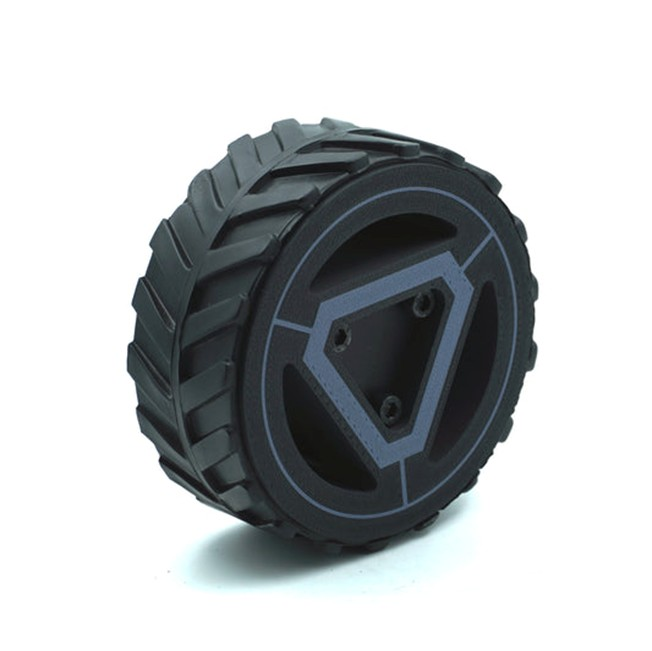
\includegraphics[height=3.5cm, keepaspectratio]{figures/Chapter 3/Standard_Fixed_wheels.jpg}
        \caption{Standard Fixed Wheels}
        \label{fig:fixed_wheels}
    \end{subfigure}
    \hfill
    \begin{subfigure}[b]{0.32\textwidth}
        \centering
        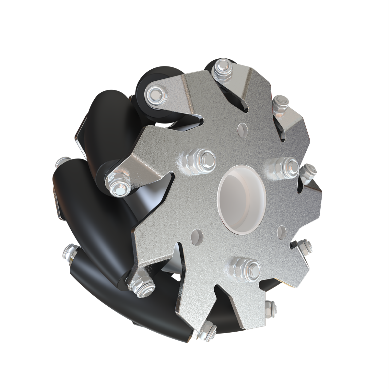
\includegraphics[height=3.5cm, keepaspectratio]{figures/Chapter 3/mecanum_wheel.png}
        \caption{Mecanum Wheel}
        \label{fig:mecanum_wheel}
    \end{subfigure}
    \hfill
    \begin{subfigure}[b]{0.32\textwidth}
        \centering
        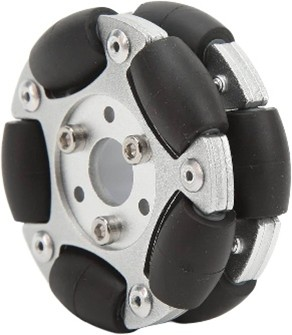
\includegraphics[height=3.5cm, keepaspectratio]{figures/Chapter 3/omnidirectional_wheel.jpg}
        \caption{Omni-Directional Wheel}
        \label{fig:omni_wheel}
    \end{subfigure}
    \caption{Robotic Wheel Technologies Comparison}
    \label{fig:wheel_technologies}
\end{figure}

\paragraph{B. Selection Criteria}
To determine the optimal wheel for our robots, seven specific criteria were established to evaluate the wheel types against the "Ausra" project requirements:
\begin{enumerate}
    \item \textbf{Holonomic Motion:} The ability to move in any direction instantly without changing the robot's heading. This is crucial for executing synchronized swarm formations.
    \item \textbf{Environment Compatibility:} Performance on flat, indoor laboratory surfaces.
    \item \textbf{Control Simplicity:} The mathematical ease of mapping desired robot velocities ($V_x, V_y, \omega$) to motor PWM signals using the ESP32.
    \item \textbf{Traction:} The grip of the wheel on the surface to prevent drifting and ensure accurate odometry feedback.
    \item \textbf{Space/Weight:} Keeping the physical footprint small to allow multiple robots to navigate tight spaces simultaneously.
    \item \textbf{Number of Wheels Needed:} This affects the complexity of the assembly and the total number of motors and motor drivers required per robot.
    \item \textbf{Unit Cost:} The financial impact of the wheel choice, which scales significantly across a swarm of three or more robots.
\end{enumerate}

\paragraph{C. Quantitative Selection Matrix}
The following selection matrix is conducted to rank each locomotion type and provide a final selection for our Ausra robots wheels for the desired motion and performance:

\begin{table}[H]
\centering
\caption{Wheel Selection Matrix}
\label{tab:wheel_matrix}
\resizebox{\textwidth}{!}{%
\begin{tabular}{|l|c|c|c|c|c|c|c|}
\hline
\multirow{2}{*}{\textbf{Criteria}} & \multirow{2}{*}{\textbf{Weights}} & \multicolumn{2}{c|}{\textbf{Standard fixed}} & \multicolumn{2}{c|}{\textbf{Mecanum}} & \multicolumn{2}{c|}{\textbf{Omni}} \\ \cline{3-8} 
 &  & Rating/5 & Score & Rating/5 & Score & Rating/5 & Score \\ \hline
Holonomic motion & 5 & 1 & 5 & 5 & 25 & 5 & 25 \\ \hline
Unit cost & 4 & 5 & 20 & 3 & 12 & 4 & 16 \\ \hline
No. of wheels & 4 & 3 & 12 & 2 & 8 & 3 & 12 \\ \hline
Env. Compatibility & 3 & 4 & 12 & 5 & 15 & 5 & 15 \\ \hline
Control Simplicity & 3 & 5 & 15 & 3 & 9 & 4 & 12 \\ \hline
Traction & 3 & 4 & 12 & 3 & 9 & 3 & 9 \\ \hline
Space/weight & 2 & 5 & 10 & 3 & 6 & 4 & 8 \\ \hline
\textbf{Final Scores} &  &  & \textbf{84} &  & \textbf{84} &  & \textbf{97} \\ \hline
\end{tabular}%
}
\end{table}

\paragraph{D. Selection Rationale}
The Omni-wheel emerged as the superior choice for the "Ausra" project with a weighted score of 97. The selection is justified by the following engineering trade-offs:
\begin{itemize}
    \item \textbf{Indoor Optimization:} As the swarm is designed for indoor buildings and laboratories, the Omni-wheel's ability to "slide" laterally on flat floors provides unmatched maneuverability without the friction and floor damage associated with Tracked systems.
    \item \textbf{The 3-Wheel Advantage:} Unlike Mecanum wheels which require a 4-wheel rectangular frame for holonomic motion, Omni-wheels allow for a 3-wheel 120\degree\ configuration. This effectively reduces the required motors and drivers by 25\% per robot.
    \item \textbf{Economic Scalability:} For a swarm of three robots, the 3-wheel Omni setup requires only 9 motors in total, whereas a Mecanum setup would require 12. This reduction in part count directly lowers the total project cost and simplifies the hardware-in-the-loop (HIL) testing phase.
    \item \textbf{Swarm Maneuverability:} The 3-DOF capability allows the "Sirius" robots to translate in any direction while rotating, which is a fundamental requirement for the high-level swarm coordination algorithms being developed for this project.
\end{itemize}

\subsubsection{Chassis Geometry \& Configuration}
The chassis serves as the structural backbone of the robot, providing the mounting surfaces for the actuation group, the electronic stack, and the perception sensors. For a three-wheel omnidirectional platform, the geometric configuration of the chassis is not merely an aesthetic choice; it dictates the robot's footprint, stability, and its "sweep area" during rotation.

\paragraph{A. Available Geometric Configurations}
Three primary geometric profiles were evaluated during the design phase, each offering distinct advantages and trade-offs regarding component density and maneuverability.

\begin{figure}[H]
    \centering
    \begin{subfigure}[b]{0.3\textwidth}
        \centering
        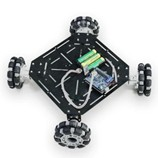
\includegraphics[width=\linewidth]{figures/Chapter 3/rectangular_square_chassis.jpg}
        \caption{Rectangular}
    \end{subfigure}
    \hfill
    \begin{subfigure}[b]{0.3\textwidth}
        \centering
        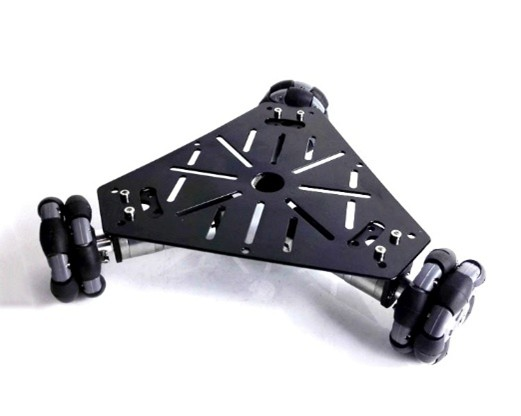
\includegraphics[width=\linewidth]{figures/Chapter 3/triangular_chassis.jpg}
        \caption{Triangular}
    \end{subfigure}
    \hfill
    \begin{subfigure}[b]{0.3\textwidth}
        \centering
        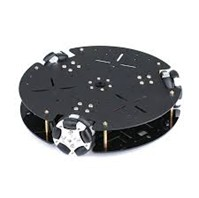
\includegraphics[width=\linewidth]{figures/Chapter 3/circular_chassis.jpg}
        \caption{Circular}
    \end{subfigure}
    \caption{Chassis Configuration Options}
    \label{fig:chassis_options}
\end{figure}

\begin{itemize}
    \item \textbf{Rectangular/Square Chassis:}
    \begin{itemize}
        \item \textbf{Description:} A four-sided frame where wheels are typically mounted at the corners.
        \item \textbf{Mechanical Profile:} This is the most common shape in robotics due to the ease of mounting rectangular PCBs and batteries. However, this profile requires a 4-wheel 90\degree\ omni-drive system like the mecanum wheel configuration. This would increase the costs significantly, especially when we scale the number of robots to 3 or 4 and each wheel requires a motor to drive it.
    \end{itemize}
    \item \textbf{Triangular Chassis:}
    \begin{itemize}
        \item \textbf{Description:} A three-sided frame, where wheels are mounted at the center of each edge or at the vertices.
        \item \textbf{Mechanical Profile:} This is the most "minimalist" design, offering the lowest weight. While it perfectly aligns with the 120\degree\ motor orientation, the tapered edges provide very little surface area for mounting high-level computing boards and sensors, which are typically rectangular. This often leads to "overhang," where sensitive electronics protrude beyond the protection of the chassis.
    \end{itemize}
    \item \textbf{Circular Chassis:}
    \begin{itemize}
        \item \textbf{Description:} A disk-shaped platform where motors are mounted 120\degree\ apart along the perimeter.
        \item \textbf{Mechanical Profile:} The circular design is the most balanced for holonomic robots. It provides a uniform radius from the center of rotation to any point on the perimeter, ensuring that the robot's footprint remains identical regardless of its heading.
    \end{itemize}
\end{itemize}

\paragraph{B. The Selection Matrix}
The configurations were scored based on the specific needs of the Sirius swarm, where multiple robots must operate in close proximity.

\begin{table}[H]
\centering
\caption{Chassis Selection Matrix}
\resizebox{\textwidth}{!}{%
\begin{tabular}{|l|c|c|c|c|c|c|c|}
\hline
\multirow{2}{*}{\textbf{Criteria}} & \multirow{2}{*}{\textbf{Weights}} & \multicolumn{2}{c|}{\textbf{Rectangular}} & \multicolumn{2}{c|}{\textbf{Circular}} & \multicolumn{2}{c|}{\textbf{Triangular}} \\ \cline{3-8} 
 &  & Rating/5 & Score & Rating/5 & Score & Rating/5 & Score \\ \hline
Mounting Surface area & 5 & 5 & 25 & 5 & 25 & 2 & 10 \\ \hline
No of wheels & 4 & 1 & 4 & 5 & 20 & 5 & 20 \\ \hline
Collision Avoidance Ease & 4 & 2 & 8 & 5 & 20 & 3 & 12 \\ \hline
Weight Efficiency & 3 & 3 & 9 & 4 & 12 & 5 & 15 \\ \hline
Structural Integrity & 3 & 5 & 15 & 4 & 12 & 3 & 9 \\ \hline
\textbf{Final Scores} &  &  & \textbf{61} &  & \textbf{89} &  & \textbf{66} \\ \hline
\end{tabular}%
}
\end{table}

\paragraph{C. Detailed Rationale for the Circular Design}
The circular geometry was selected as the optimal chassis configuration for the following engineering reasons:
\begin{enumerate}
    \item \textbf{Constant Sweep Area (Rotational Symmetry):} In swarm robotics, collision avoidance is a primary challenge. A circular chassis has a constant radius ($R$). This means that if the robot rotates in place, its "occupancy" in the 2D map does not change. Unlike a rectangular or triangular robot—which might hit an obstacle only when it turns—the circular Sirius robot can rotate freely without increasing its risk of collision. This simplifies the navigation algorithms significantly.
    \item \textbf{Optimized Internal "Real Estate":} The graduation project requires a significant hardware stack: a microcontroller, motor drivers, a high-level computing board, a battery, a 2D lidar, and the depth camera. A circular plate with a 30 cm diameter provides a much larger surface area than a triangular plate of the same width. This allows for a "cleaner" layout, better cable management, and the ability to mount components centrally to keep the Center of Gravity (CoG) perfectly aligned with the center of rotation.
    \item \textbf{Mechanical Stability \& Load Distribution:} The 120\degree\ motor placement on a circular disk ensures that the load is distributed evenly across all three points of contact. In a triangular design, the "sharp" corners are structural weak points; in a circular design, the stress from the motor mounts is distributed more uniformly along the arc of the plate, reducing the risk of material fatigue or warping over time.
    \item \textbf{Aesthetic and Functional Uniformity:} As a swarm of three autonomous robots, uniformity is key. The circular design allows for a modular "stack" where each layer (Base, Control, Perception) can be identical across all three units, facilitating interchangeable parts and easier mass assembly.
\end{enumerate}

\newpage
\subsubsection{Material Selection of Robot Plate}
In this section we will discuss the Robot Plate material selection.

\paragraph{A. Available Materials}
After a lot of surveying and discussion in choosing the best materials in the market and through our research that could be used for our Robot that satisfies our targets. We will discuss the available options, their associated advantages and disadvantages, and how they interact to providing the desired performance.

\begin{table}[H]
    \centering
    \caption{Available Materials}
    \begin{tabular}{|l|c|c|c|l|}
    \hline
    \textbf{Material} & \textbf{Yield Stress (MPa)} & \textbf{Density (Kg/m$^3$)} & \textbf{Young’s Modulus (Gpa)} & \textbf{Price} \\
    \hline
    Aluminum & 100-500 & 2700 & 69 & Mod. High \\
    \hline
    Acrylic & 60-80 & 1200 & 3.2 & Moderate \\
    \hline
    Steel & 250-700 & 7900 & 200 & Moderate \\
    \hline
    \end{tabular}
\end{table}

Using Steel for the plates in the robot is a strong and durable choice. It’s tough and doesn’t easily get deflected plus it’s not too expensive. The disadvantage of it is that it’s too heavy to be used in our Robots.

Aluminum is a good choice for our Robots but, it has downside of having a high cost between the other two options, as it good in part of being relatively low in weight and rigid enough.

Last for Acrylic is the lowest in strength, can crack under impact or stress concentrations, but have the lowest weight and used as insulator that won’t cause shorts and lowest in the price.

\paragraph{B. Plate Material selection Matrix}
For swarm robots weight is critical for battery life and mobility. Our target here is to select the most suitable material to meet our defined targets.

\begin{table}[H]
\centering
\caption{Plate Material Selection Matrix}
\resizebox{\textwidth}{!}{%
\begin{tabular}{|l|c|c|c|c|c|c|c|}
\hline
\multirow{2}{*}{\textbf{Criteria}} & \multirow{2}{*}{\textbf{Weights}} & \multicolumn{2}{c|}{\textbf{Steel}} & \multicolumn{2}{c|}{\textbf{Aluminum}} & \multicolumn{2}{c|}{\textbf{Acrylic}} \\ \cline{3-8} 
 &  & Rating/5 & Score & Rating/5 & Score & Rating/5 & Score \\ \hline
Stiffness to Weight Ratio & 4 & 5 & 20 & 4 & 16 & 2 & 8 \\ \hline
Manufacturability & 5 & 4 & 20 & 5 & 25 & 5 & 25 \\ \hline
Price & 4 & 5 & 20 & 3 & 12 & 5 & 20 \\ \hline
Density & 5 & 1 & 5 & 4 & 20 & 5 & 25 \\ \hline
\textbf{Final Scores} &  &  & \textbf{65} &  & \textbf{73} &  & \textbf{78} \\ \hline
\end{tabular}%
}
\end{table}

Based on the selection matrix table resulted in that Acrylic is the best option for its weight over steel and aluminum in density and Manufacturability although it has the least score in stiffness to weight Ratio, but we will approve it’s durability in stress analysis.

\newpage

\subsubsection{Evaluation of Materials}
The main structural component of the robot is a cylindrical “wall” of housing that serves as the backbone for all internal components, sensors, and the three-omni-wheel drivetrain. The material must resist warping while staying within the 5kg mass constraint.
These materials were evaluated for the construction of cylindrical housing: PLA (3D-printed), Sheet metal (Aluminum).

\begin{figure}[H]
    \centering
    \begin{subfigure}[b]{0.45\textwidth}
        \centering
        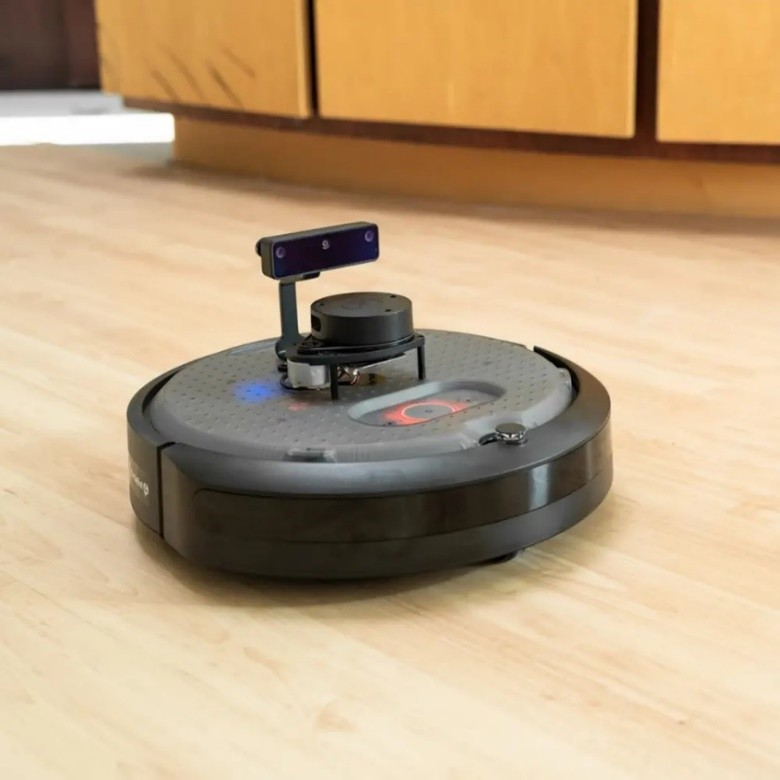
\includegraphics[width=\linewidth]{figures/Chapter 3/Inspiration_design_for_the_chasis_v1.jpg}
        \caption{Design Inspiration V1}
    \end{subfigure}
    \hfill
    \begin{subfigure}[b]{0.45\textwidth}
        \centering
        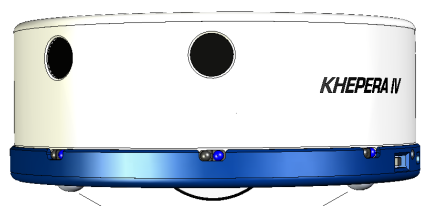
\includegraphics[width=\linewidth]{figures/Chapter 3/Inspiration_design_for_the_chasis_v2.png}
        \caption{Design Inspiration V2}
    \end{subfigure}
    \caption{Inspiration Design for The Chassis}
    \label{fig:chassis_inspiration}
\end{figure}


\paragraph{Candidate Materials Analysis}
\begin{enumerate}
    \item \textbf{3D-Printed Polylactic Acid (PLA):} PLA is the most versatile option for rapid prototyping. It allows for the creation of complex internal fixations and integrated sensor mounts that would be impossible to manufacture with traditional methods.
    \item \textbf{Aluminum Sheet Metal (6061 Alloy):} Aluminum offers the highest strength-to-weight ratio and provides excellent protection for internal electronics.
\end{enumerate}

\paragraph{Material Selection Matrix}

\begin{table}[H]
\centering
\caption{Chassis Construction Selection Matrix}
\begin{tabular}{|l|c|c|c|c|c|}
\hline
\multirow{2}{*}{\textbf{Criteria}} & \multirow{2}{*}{\textbf{Weights}} & \multicolumn{2}{c|}{\textbf{Sheet Metal Aluminum}} & \multicolumn{2}{c|}{\textbf{PLA-3D-Printed}} \\ \cline{3-6} 
 &  & Rating/5 & Score & Rating/5 & Score \\ \hline
Manufacturability & 5 & 3 & 15 & 5 & 25 \\ \hline
Rigidity & 4 & 5 & 20 & 3 & 12 \\ \hline
Internal Fixation Integration & 3 & 3 & 9 & 4 & 12 \\ \hline
Weight & 3 & 4 & 12 & 5 & 15 \\ \hline
\textbf{Final Scores} &  &  & \textbf{56} &  & \textbf{64} \\ \hline
\end{tabular}
\end{table}

Based on the selection matrix above, the 3D-printed PLA was selected as the primary material for the cylindrical wall and internal fixations. The deciding factor was the integration of complex geometry.
Since the robot utilizes a 3-omni-wheel configuration, the motor mounts must be positioned at exactly 120\degree\ intervals.


\subsubsection{Actuator Sizing and Motor Selection}
The selection of actuators is a critical phase in the mechanical design of the Ausrabot robot. The motors must provide sufficient torque to overcome static friction and inertia while maintaining a rotational speed that meets the minimum linear velocity requirement of 0.2 m/s. This section outlines the requirements determined by the robot's kinematics and justifies the final component choice through a weighted selection matrix.

\paragraph{A. Determination of Motor Requirements}
To size the actuators correctly, the desired robot performance must be mapped to the individual wheel requirements. Unlike a standard differential drive, a 3-wheel omni-directional configuration at dictates that wheel speeds are vector components of the robot’s total velocity.
\begin{enumerate}
    \item \textbf{Kinematic Velocity Requirements:} For a robot to achieve a translational velocity of 0.2 m/s, the individual wheel speeds must account for the geometry of the 120 degree configuration of the omni wheels. As detailed in the Kinematics Section, the relationship between the robot velocity and individual wheel velocity is defined by the transformation matrix. To ensure the robot can reach 0.2 m/s in any direction and maintain rotational stability:
    \begin{itemize}
        \item \textbf{Calculated Minimum Motor RPM:} Considering the wheel radius (r = 0.0325m) and the kinematic constraints, the motors must provide a rated speed of at least 85–90 RPM.
        \item \textbf{Target Linear Velocity (v):} > 0.2 m/s.
    \end{itemize}
    \item \textbf{Torque Requirements:} The motor must overcome the Force of Inertia ($F_i$) and the Rolling Resistance ($F_{rr}$). Given the Nylon rollers of the Omni-wheels on indoor flooring, a rolling resistance coefficient ($C_{rr}$) of 0.02 is assumed for a maximum robot mass of 5 kg.
    \begin{itemize}
        \item \textbf{Total Force ($F_{total}$):} Approximately 1.98 N (calculated from $m a + m g C_{rr}$).
        \item \textbf{Required Rated Torque:} To handle the 5 kg payload and provide a safety margin for slopes or surface irregularities, the motors must provide a rated torque of at least 0.8–1.0 kg·cm.
    \end{itemize}
\end{enumerate}

\paragraph{B. Comparative Analysis of Available Actuators}
Three motors were evaluated based on the 12V power constraint and the physical requirements of the swarm units.

\begin{enumerate}
    \item \textbf{JGA25-370 (High Speed, 130 RPM):} A standard spur-geared DC motor. While it offers high speed and a compact form factor, it possesses lower torque compared to worm-gear alternatives, which may struggle with the maximum 5 kg payload.
    \item \textbf{JGY-370-1285 (Worm Gear, 98 RPM):} This motor features a worm-gear reduction which provides significantly higher torque and a self-locking mechanism. The 98 RPM output perfectly matches the required range determined by the kinematic analysis while ensuring high pushing force.
    \item \textbf{E-S Planetary Geared Motor (182 RPM):} A high-performance planetary motor. While technically superior in speed, its physical length > 90mm with encoder) combined with the omni wheel, coupler, shaft, bearing and brackets would cause the robot's total radius to exceed the 0.3m (30 cm) limit established in the design requirements.
\end{enumerate}

\begin{figure}[H]
    \centering
    \begin{subfigure}[b]{0.32\textwidth}
        \centering
        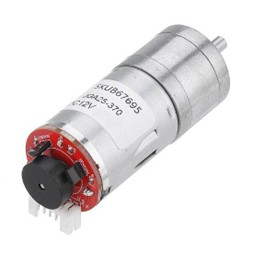
\includegraphics[width=\linewidth]{figures/Chapter 3/JGA25-370_motor.jpg}
        \caption{JGA25-370}
        \label{fig:jga25}
    \end{subfigure}
    \hfill
    \begin{subfigure}[b]{0.32\textwidth}
        \centering
        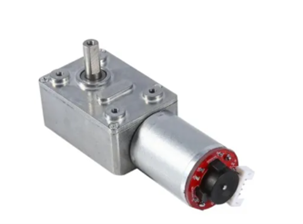
\includegraphics[width=\linewidth]{figures/Chapter 3/JGY-370-1285_motor.png}
        \caption{JGY-370 (Worm)}
        \label{fig:jgy370}
    \end{subfigure}
    \hfill
    \begin{subfigure}[b]{0.32\textwidth}
        \centering
        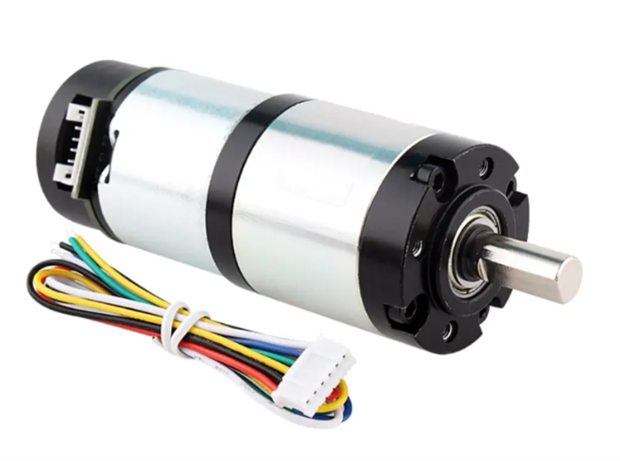
\includegraphics[width=\linewidth]{figures/Chapter 3/E-S_Planetary_Geared_Motor.png}
        \caption{E-S Planetary}
        \label{fig:es_planetary}
    \end{subfigure}
    \caption{Comparative view of evaluated motors}
    \label{fig:motor_comparison}
\end{figure}

\paragraph{C. Actuator Selection Criteria}
To objectively determine the best actuator for the swarm, five key criteria were established:
\begin{enumerate}
    \item \textbf{Torque Performance (Weight 5):} The ability of the motor to drive a 5 kg robot consistently without overheating or stalling, especially during high-torque swarm maneuvers.
    \item \textbf{Size/Footprint (Weight 5):} The physical length and mounting orientation must allow the three motors to be placed 120 apart without exceeding the 30 cm robot diameter limit.
    \item \textbf{Speed/RPM (Weight 4):} The motor must meet or exceed the 85-90 RPM threshold to maintain the 0.2 m/s target velocity across all translation vectors.
    \item \textbf{Self-Locking/Stability (Weight 3):} The inherent ability of the gear system to hold its position when unpowered. This is vital for static mapping and station-keeping in a swarm.
    \item \textbf{Unit Cost (Weight 2):} Since the project involves a swarm of three robots (requiring 9 motors in total), the individual price per unit is a significant factor in the overall project budget.
\end{enumerate}

\paragraph{D. Selection Matrix}
The following matrix evaluates the motors against the project constraints. For "Torque Performance," the highest weight is assigned as it is critical for handling the 5 kg design limit.

\begin{table}[H]
\centering
\caption{Motor Selection Matrix}
\resizebox{\textwidth}{!}{%
\begin{tabular}{|l|c|c|c|c|c|c|c|}
\hline
\multirow{2}{*}{\textbf{Criteria}} & \multirow{2}{*}{\textbf{Weights}} & \multicolumn{2}{c|}{\textbf{JGA25-370}} & \multicolumn{2}{c|}{\textbf{JGY-370 (Worm)}} & \multicolumn{2}{c|}{\textbf{E-S Planetary}} \\ \cline{3-8} 
 &  & Rating/5 & Score & Rating/5 & Score & Rating/5 & Score \\ \hline
Torque Performance & 5 & 2 & 10 & 4 & 20 & 5 & 25 \\ \hline
Size/Footprint & 4 & 4 & 16 & 3 & 12 & 1 & 4 \\ \hline
Speed/RPM & 4 & 4 & 16 & 3 & 12 & 5 & 20 \\ \hline
Self-Locking /Stability & 3 & 2 & 6 & 4 & 12 & 3 & 9 \\ \hline
Unit cost & 3 & 5 & 15 & 5 & 15 & 2 & 6 \\ \hline
\textbf{Final Scores} &  &  & \textbf{63} &  & \textbf{71} &  & \textbf{64} \\ \hline
\end{tabular}%
}
\end{table}

\paragraph{E. Selection Rationale}
The JGY-370 Worm Gear motor (98 RPM) was selected as the optimal actuator for the Ausra robot.
The primary driver for this selection was the high rated torque provided by the worm-gear reduction. As the robot is designed for a maximum mass of 5 kg, the JGA25-370 was deemed insufficient for reliable long-term operation under full load. The JGY-370's 98 RPM speed is well-optimized for the 3-wheel kinematics, providing enough headroom to achieve the 0.2 m/s target velocity without excessive power consumption.
A unique advantage of the JGY-370 is its self-locking property. In a swarm environment, the ability of the robot to maintain its position without consuming power (braking) is highly beneficial for static 2D mapping tasks and formation holding. Although the worm-gear orientation requires careful mounting, it fits within the 30 cm radius constraint, unlike the E-S Planetary motor which was rejected for its prohibitive length and high unit cost.


\newpage

\section{Detailed CAD Design}
\label{sec:cad_design}

\subsection{CAD Modeling \& Geometry}
The physical realization of the Ausra robot follows modular "Tri-Level Stack" architecture. This design allows for a clear separation between high-current power systems, low-level control logic, and high-level perception hardware. The assembly was modeled in SolidWorks to ensure precise tolerances, specifically for the radial symmetry of the locomotion system. The assembly of the full robot is based on mounting all the hardware components we selected previously.

\begin{figure}[H]
    \centering
    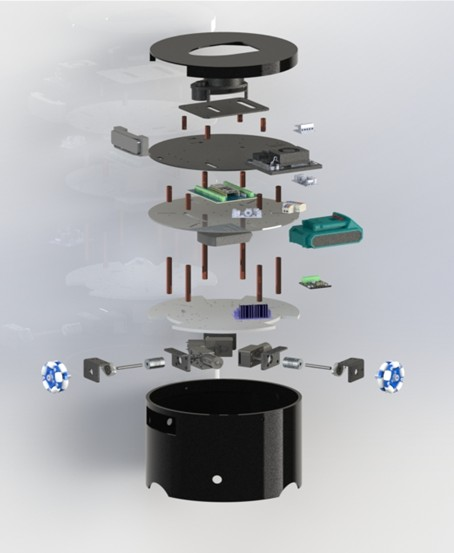
\includegraphics[width=0.8\linewidth]{figures/Chapter 3/vertical_exploded_view.jpg}
    \caption{Vertical Exploded View of the Robot Stack}
    \label{fig:exploded_stack}
\end{figure}

\newpage

\subsubsection{Layer 1: The Locomotion \& Power Drive Base Plate}
The first layer of the Ausra robot acts as the structural and mechanical foundation of the entire system. Its primary role is to serve as a rigid, high-torque platform that translates digital control vectors into physical movement. In an omni-directional swarm robot, the base plate must not only support the static weight of the upper electronics stack but also withstand the dynamic, multi-directional forces generated during rapid translations and rotations. Consequently, the design of this layer focuses heavily on structural rigidity, mechanical load distribution, and power transmission integrity.

\begin{figure}[H]
    \centering
    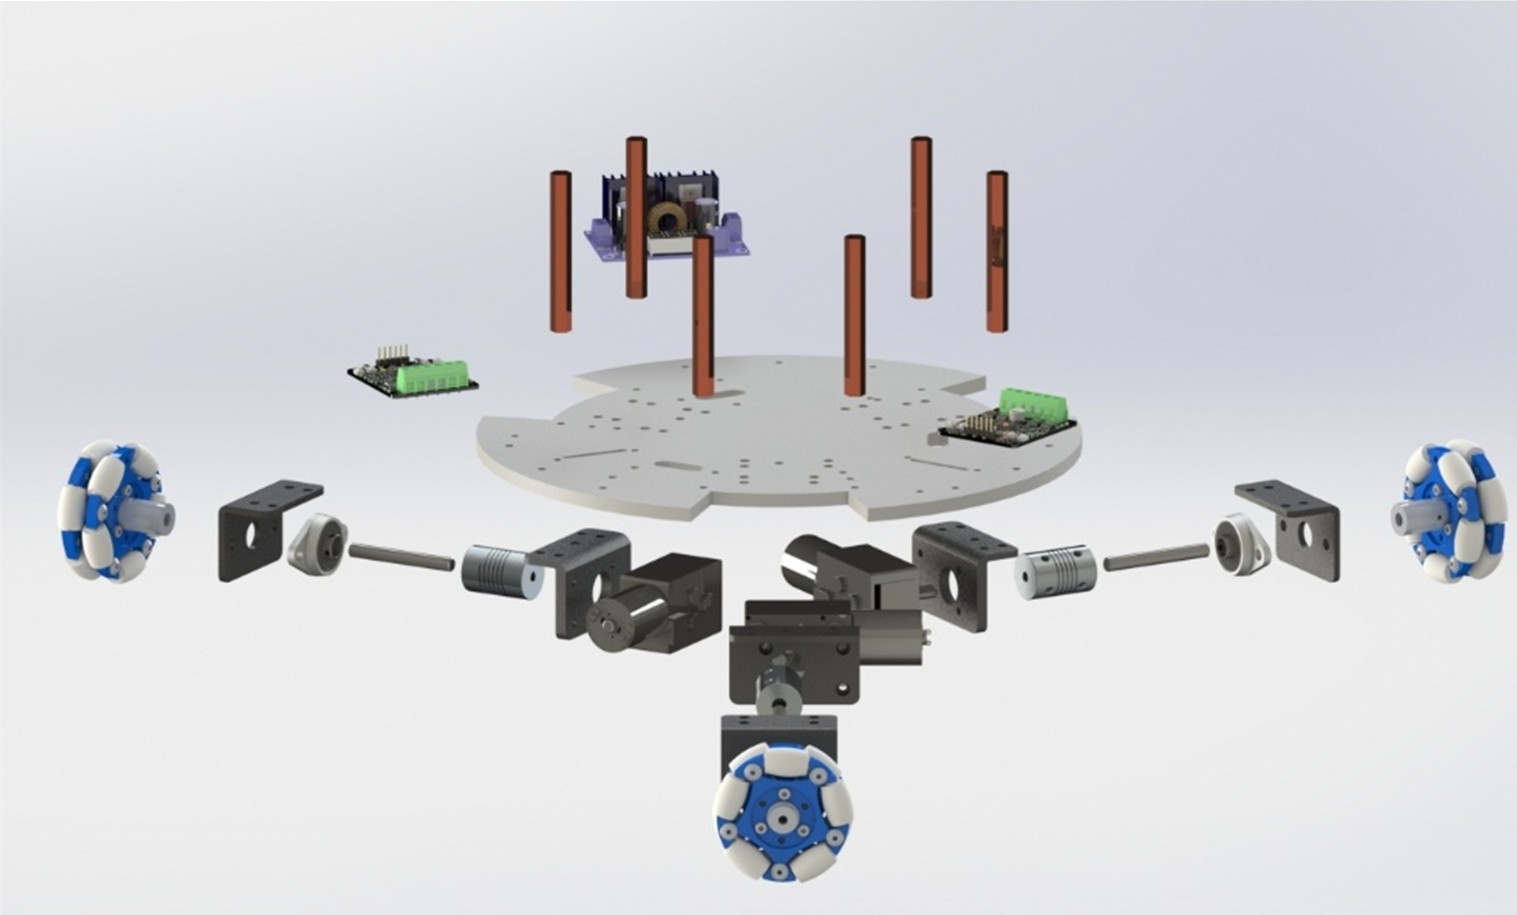
\includegraphics[width=\linewidth]{figures/Chapter 3/Locomotion_and_Power_Drive_Base_Plate_exploded_view.jpg}
    \caption{Base Plate Exploded View}
    \label{fig:base_plate}
\end{figure}

\newpage
\paragraph{A. The Actuation Assembly and Radial Support System}
A common failure point in mobile robotics is the excessive radial load applied directly to motor shafts, especially during the lateral "sliding" maneuvers typical of omni-directional movement. To ensure the longevity of the JGY-370 worm-gear motors, a sophisticated dual-point support system was engineered. Each motor is anchored to the base plate using high-strength motor brackets positioned at precise radial intervals. This symmetry is critical for maintaining balanced kinematics and a centralized center of mass.
However, the standout feature of this layer is the auxiliary bearing support system. Unlike hobby-grade designs where wheels are cantilevered directly off the motor gearbox, the Ausra robot utilizes an additional bearing bracket for each drive line. This bracket houses a precision ball bearing that supports the end of the driveshaft just before it interfaces with the wheel. By introducing this second point of contact, any bending moments or perpendicular shocks encountered by the wheels are absorbed by the bearing and the chassis plate itself, rather than the motor’s internal brass gears. This mechanical isolation significantly reduces the risk of shaft deformation and gear stripping, ensuring the robot remains operational under its maximum 5kg payload.

\begin{figure}[H]
    \centering
    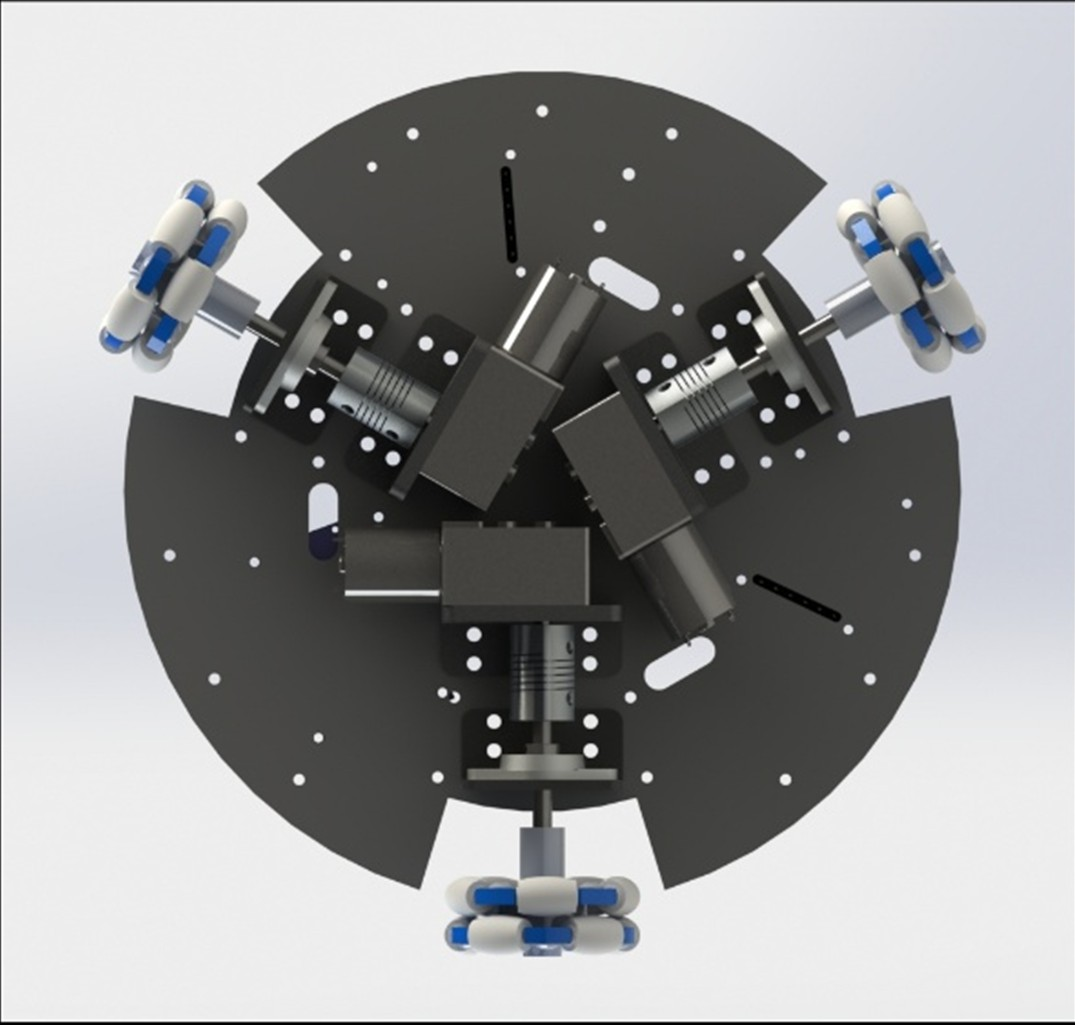
\includegraphics[width=0.9\linewidth]{figures/Chapter 3/Actuation_Assembly_and_Radial_Support_System.jpg}
    \caption{Actuation Assembly and Radial Support}
    \label{fig:radial_support}
\end{figure}

\paragraph{B. Precision Power Transmission and Coupling}
To bridge the gap between the centrally mounted motors and the peripheral Omni-wheels, a robust power transmission line was implemented. Each drive line utilizes a precision-ground steel driveshaft with a length of 50 mm and a diameter of 8mm. Steel was selected specifically for its high torsional rigidity; it ensures that the shaft can transmit the high stall torque of the worm-gear reduction without twisting or flexing, which would otherwise introduce inaccuracies in the robot's odometry and SLAM data.
The transmission is managed through a dual-coupling strategy designed for zero-slip performance. A primary coupler interfaces the 6 mm D-shaped output of the motor to the 8 mm steel shaft. At the distal end, an Aluminum wheel coupler secures the shaft to the Omni-wheel. Aluminum was chosen for the wheel interface because it provides a lightweight yet durable "bite" on the shaft. These couplers are secured using industrial-grade set-screws, ensuring that every rotation of the motor is perfectly mirrored by the wheel—a fundamental requirement for the high-precision coordination needed in swarm formations.

\begin{figure}[H]
    \centering
    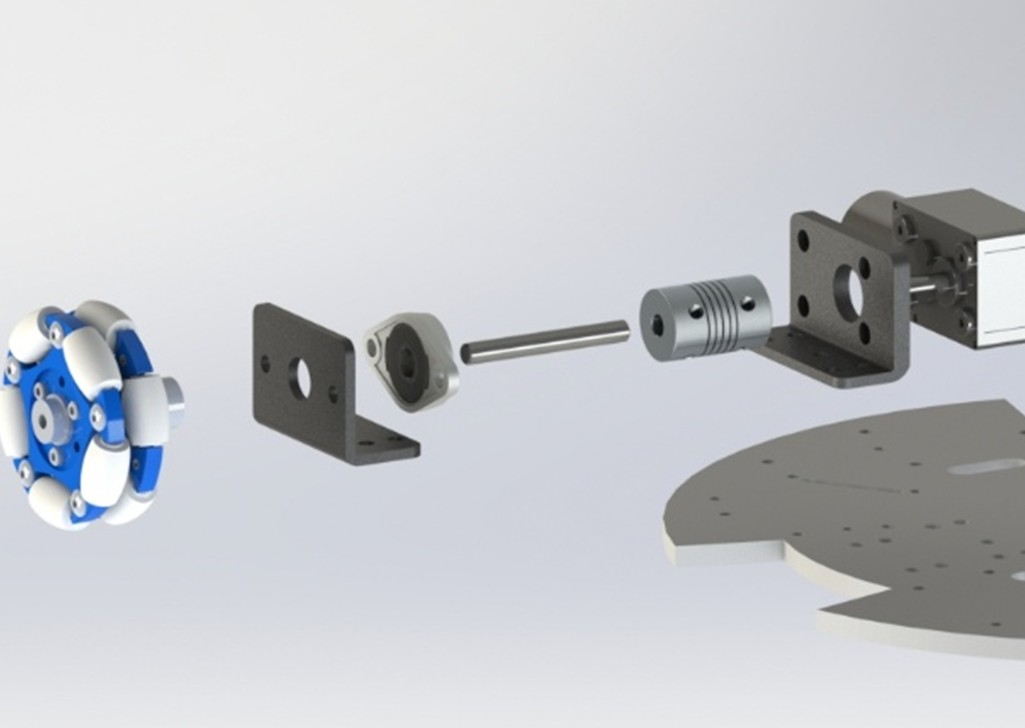
\includegraphics[width=0.6\linewidth]{figures/Chapter 3/Precision_Power_Transmission_and_Coupling.jpg}
    \caption{Precision Power Transmission and Coupling}
    \label{fig:power_trans}
\end{figure}

\paragraph{C. Integrated Power Control and Signal Integrity}
The top surface of the first layer functions as the high-current "Engine Room" of the robot. To protect the sensitive perception sensors and microcontrollers on the upper layers from Electromagnetic Interference (EMI) and electrical noise, the high-power components are localized here. Two Cytron motor drivers are mounted directly to the base plate, positioned in close proximity to the actuators. This strategic placement minimizes the length of high-current wiring, which in turn reduces voltage drops and parasitic inductance that can occur during rapid motor reversals.
Furthermore, this layer includes a dedicated Buck Converter specifically for logic regulation. This converter steps down the main 12V battery supply to a stable logic-level voltage for the motor drivers. By isolating the driver logic with a dedicated regulator on the base layer, the system gains a layer of protection against "brownouts." Even during peak current draws—such as when the robot must overcome high static friction—the drivers' logic remains stable, ensuring the ESP32 always maintains consistent control over the actuators.

\begin{figure}[H]
    \centering
    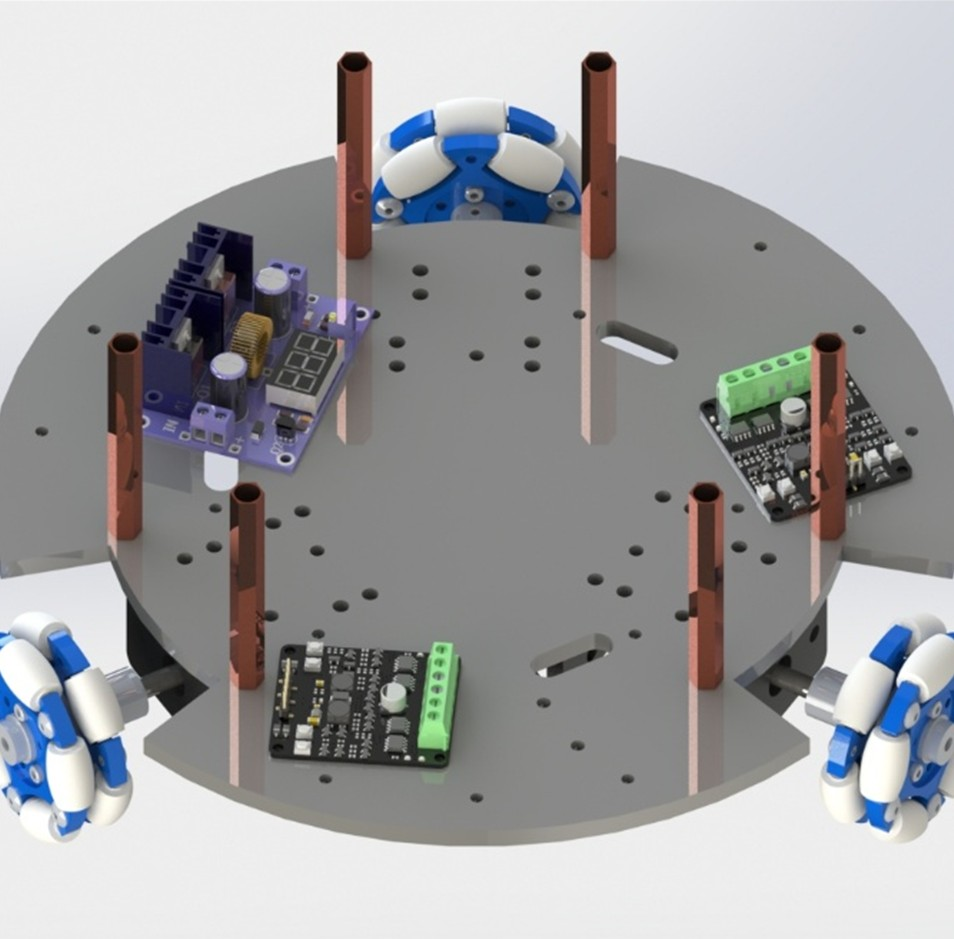
\includegraphics[width=0.6\linewidth]{figures/Chapter 3/Integrated_Power_Control_and_Signal_Integrity.jpg}
    \caption{Integrated Power Control and Signal Integrity}
    \label{fig:power_control}
\end{figure}

\subsubsection{Layer 2: Energy Storage \& Signal Processing}
The middle layer of the Sirius robot serves as the "Nervous System" of the platform, acting as the primary junction between the high-current actuation base and the high-level perception stack. Physically, this layer is designed to manage the robot's mass distribution and signal routing. By isolating the microcontroller and power distribution hardware on a dedicated central plate, the design achieves a "buffer zone" that protects sensitive logic signals from the mechanical vibrations of the base and the electromagnetic noise generated by the motors.

\begin{figure}[H]
    \centering
    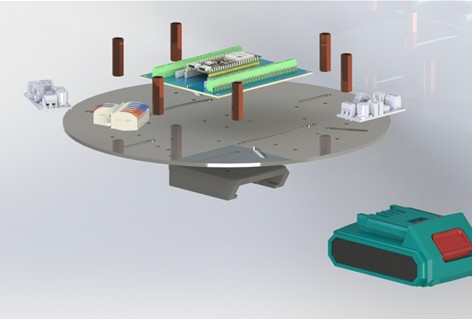
\includegraphics[width=0.6\linewidth]{figures/Chapter 3/Layer_2-_Energy_Storage_and_Signal_Processing.jpg}
    \caption{Layer 2: Energy Storage and Signal Processing}
    \label{fig:layer2_iso}
\end{figure}

\paragraph{A. Battery and Center of Gravity (CoG) Optimization}
One of the most critical factors in the stability of a three-wheeled omni-directional robot is the management of its Center of Gravity (CoG). Because the robot is capable of instantaneous acceleration in any direction, a high CoG would lead to significant tipping moments, causing the wheels to lose traction or the odometry to drift. To mitigate this, the primary energy source (Battery) is secured to the bottom surface of Layer 2.
The battery is housed within a custom-fit, 3D-printed holder designed to prevent any lateral shifting during high-G maneuvers. By mounting the heaviest single component of the robot as low as possible within the central stack, the design ensures a low CoG. This placement provides a stabilizing effect, allowing the robot to execute sharp, high-speed translations while maintaining a level profile. This physical stability is not just a mechanical preference; it is a prerequisite for the high-level SLAM algorithms, which require a stable platform to generate consistent 2D point clouds and depth maps.

\begin{figure}[H]
    \centering
    \begin{subfigure}[b]{0.45\textwidth}
        \centering
        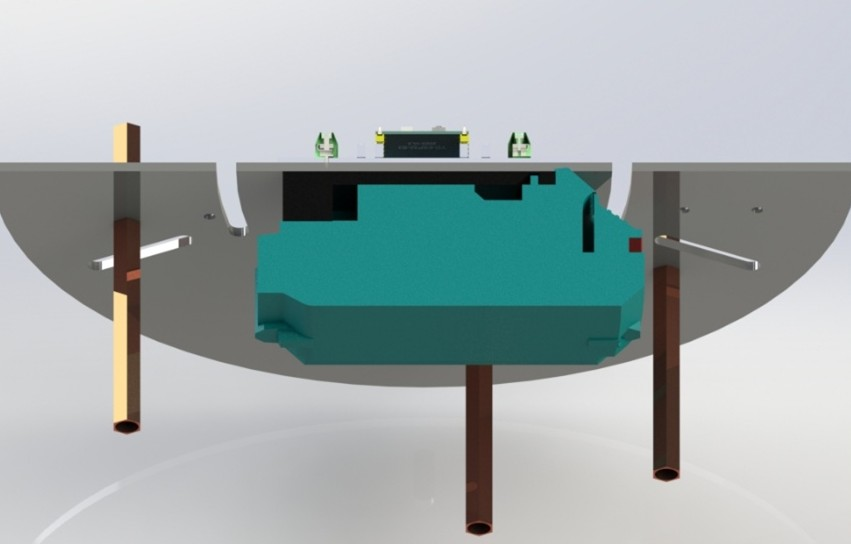
\includegraphics[width=\linewidth]{figures/Chapter 3/Battery_hub_v1.jpg}
        \caption{Battery Hub V1}
    \end{subfigure}
    \hfill
    \begin{subfigure}[b]{0.45\textwidth}
        \centering
        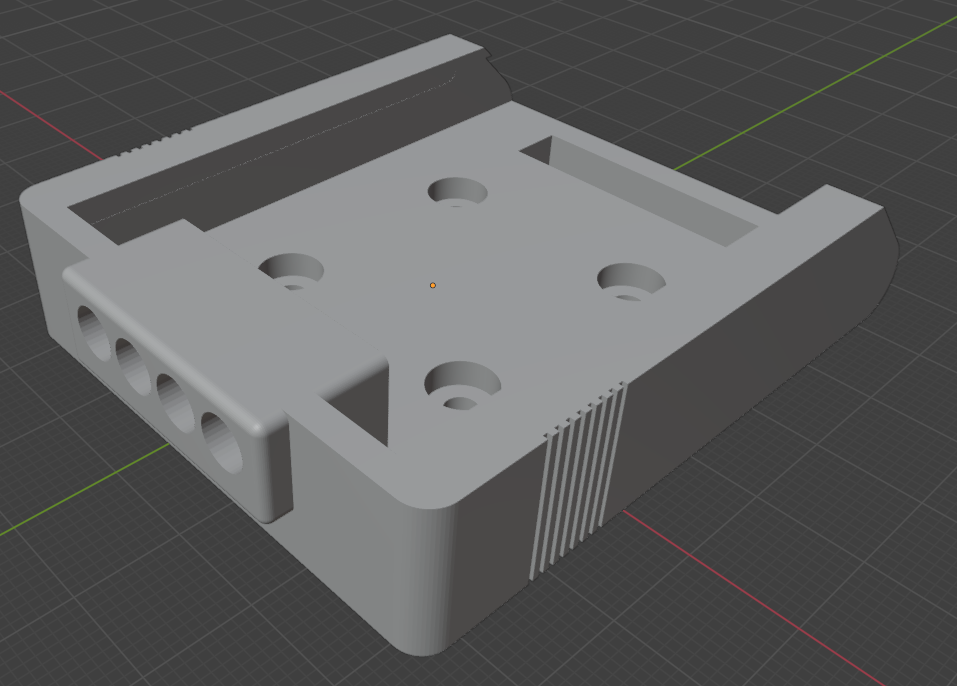
\includegraphics[width=\linewidth]{figures/Chapter 3/battery_hub_3d_printed.png}
        \caption{3D Printed Hub}
    \end{subfigure}
    
    \vspace{1em}
    
    \begin{subfigure}[b]{0.5\textwidth}
        \centering
        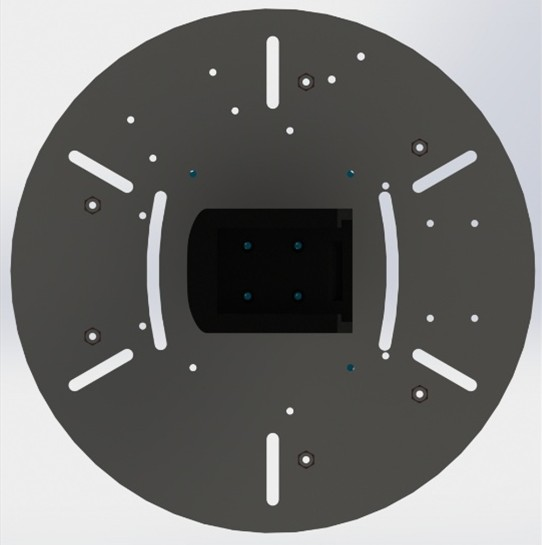
\includegraphics[width=\linewidth]{figures/Chapter 3/COG.jpg}
        \caption{Center of Gravity}
    \end{subfigure}
    
    \caption{Battery Housing and COG Optimization}
    \label{fig:battery_cog}
\end{figure}

\paragraph{B. The Centralized Control Hub and Signal Routing}
The top surface of the second layer is dedicated to the Low-Level Control Group. This hub is centered around the ESP32 microcontroller and its accompanying shield. The shield is a vital component of the "Ausra" architecture, as it allows for secure, vibration-resistant connections for the encoders and motor driver headers. By elevating the microcontroller to the second layer, we provide it with a clear physical separation from the high-current cabling of the base, significantly reducing the risk of "crosstalk" or signal corruption that could lead to erratic motor behavior.
In addition to the microcontroller, this surface hosts several critical power management components:
\begin{itemize}
    \item \textbf{Secondary Buck Converter:} While the first layer uses a regulator for motor logic, this secondary converter is dedicated exclusively to the "clean" 5V and 3.3V rails needed by the ESP32 and auxiliary sensors. This dual-regulator strategy prevents the high-frequency switching noise of the motor drivers from reaching the logic-level processors.
    \item \textbf{Main Power Switch:} Integrated directly into the plate’s perimeter for easy access, the switch provides a physical "hard-cut" for the entire system, ensuring safety during testing and maintenance.
    \item \textbf{SPL Connector Block:} The "Sirius" robot utilizes a "Star Topology" for power distribution rather than daisy-chaining components. The SPL connector acts as a centralized manifold, taking the raw battery voltage and neatly dividing it between the functional layers. This ensures that a failure or short circuit in one subsystem is less likely to affect the others, while also facilitating much cleaner cable management throughout the internal stack.
\end{itemize}
By consolidating these components on Layer 2, the design achieves a modular "Plug-and-Play" architecture. This arrangement allows a researcher to troubleshoot the control logic or swap the battery without needing to dismantle the perception sensors on the top layer or the motor mounts on the base, directly fulfilling the project’s requirement for high serviceability.

\begin{figure}[H]
    \centering
    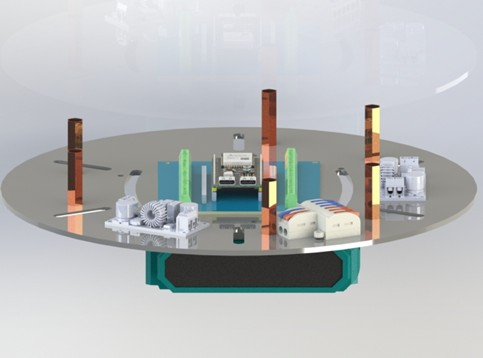
\includegraphics[width=0.7\linewidth]{figures/Chapter 3/Layer_2_assembeled.jpg}
    \caption{Assembled Layer 2 Control Hub}
    \label{fig:layer2_assembled}
\end{figure}

\subsubsection{Layer 3: Perception \& High-Level Intelligence}
The third and final layer of the Ausra robot represents the "apex" of its design, both physically and functionally. While the lower layers handle the brute force of locomotion and the steady logic of power management, the third layer is dedicated entirely to perception, spatial reasoning, and high-level autonomous decision-making. Positioned at the highest point of the stack, this layer provides the sensors with an unobstructed view of the environment, which is paramount for a swarm system tasked with collaborative 2D and 3D mapping.

\paragraph{A. High-Level Computing and Spatial AI Integration}
At the heart of this layer sits the NVIDIA Jetson Orin Nano, which serves as the robot’s primary processing unit. By mounting the Jetson centrally on the top plate, the design ensures that its heat sink remains exposed to ambient air for better thermal management while keeping its mass balanced over the robot's center of rotation. This board runs the heavy ROS2 (Robot Operating System 2) stack, orchestrating the complex communication between individual swarm members and processing the high-bandwidth data coming from the perception sensors.
Adjacent to the computing board is the OAK-D camera, the robot's primary source of "Spatial AI." In this project, the camera isn't just a passive video feed; it is used to perform real-time object detection and depth estimation. To ensure the reliability of this data, the camera is secured via a custom-designed, 3D-printed vibration-dampening holder. This holder is critical because even minor vibrations from the omni-wheels could introduce "jitter" into the depth frames, leading to errors in the SLAM (Simultaneous Localization and Mapping) process. The camera is strategically positioned at the very edge of the plate, angled to maximize its field of view without the robot's own chassis obscuring the "vision" of the lower-plane obstacles.

\paragraph{B. Navigation Sensors and SLAM Hardware}
To achieve precise 2D mapping, the Ausra robot relies on the fusion of LiDAR and inertial data. The mounting strategy for these components on the third layer is driven by the need for geometric accuracy:
\begin{itemize}
    \item \textbf{Elevated LiDAR Platform:} The LiDAR unit is the "eyes" of the 2D SLAM system. To prevent the laser from hitting the robot’s internal components or the protective outer shell, it is mounted on an elevated, secondary plate. This elevation ensures a completely unobstructed 360\degree\ horizontal scan, allowing the robot to detect walls, furniture, and other swarm members at a distance without "blind spots" created by its own structure.
    \item \textbf{Precision IMU Placement:} Orientation data is handled by the Inertial Measurement Unit (IMU), which is fixed to a small, dedicated PCB. For a mechatronics platform, the placement of the IMU is vital; it is mounted as close as possible to the robot's vertical axis of rotation. This minimizes "centripetal acceleration" noise the false readings that occur when an IMU is mounted far from the center ensuring that when the robot spins in place, the orientation data remains clean and drift-free.
\end{itemize}

\begin{figure}[H]
    \centering
    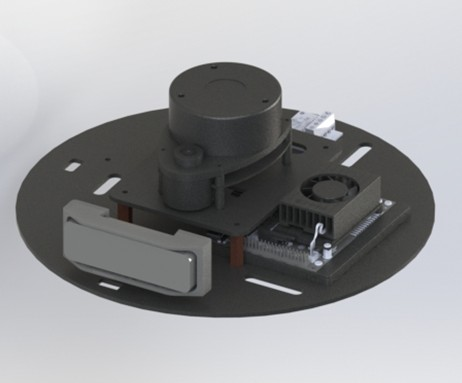
\includegraphics[width=\linewidth]{figures/Chapter 3/layer_3_assembeled.jpg}
    \caption{Assembled Layer 3 Perception Stack}
    \label{fig:layer3_assembled}
\end{figure}


\newpage
\subsubsection{Protective Enclosure (The Outer Shell \& Top Cover)}
Surrounding these three layers is an external wall and cover made from 3D-printed PLA. From a design standpoint, this shell serves two purposes: protecting the sensitive internal electronics from external impacts and providing a clean, aesthetic finish to the swarm unit. Recognizing the need for frequent hardware adjustments during the research phase, the shell was designed as a "split-shell" system. It consists of 2 parts that lock together. This allows us to remove half of the shell to access the Jetson’s ports or the ESP32’s micro-USB connection on the layer below without having to fully disassemble the robot or disturb the calibration of the LiDAR and camera on the top plate.
This layering strategy ensures that the Ausra robot is not just a collection of parts, but a highly organized, modular system where each component is placed specifically to optimize its functional performance and ease of maintenance.

\begin{figure}[H]
    \centering
    \begin{subfigure}[b]{0.45\textwidth}
        \centering
        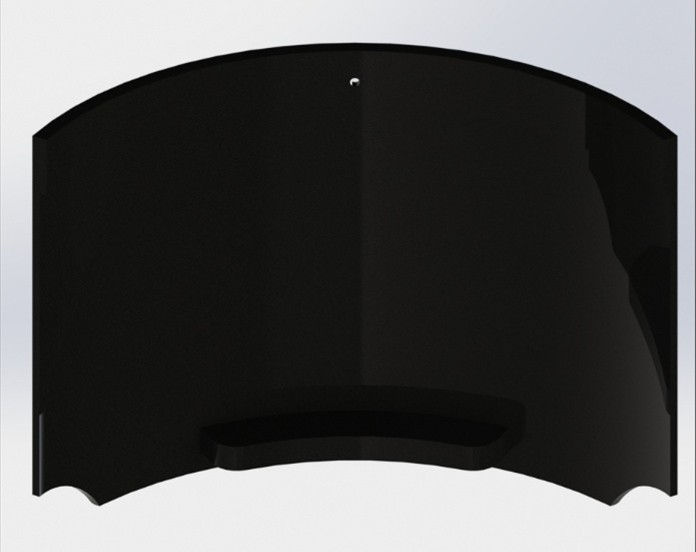
\includegraphics[width=\linewidth]{figures/Chapter 3/3d_printed_enclosure_v1.jpg}
        \caption{Part 1}
    \end{subfigure}
    \hfill
    \begin{subfigure}[b]{0.45\textwidth}
        \centering
        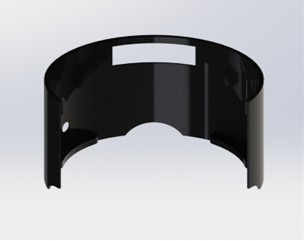
\includegraphics[width=\linewidth]{figures/Chapter 3/3d_printed_enclosure_v2.jpg}
        \caption{Part 2}
    \end{subfigure}
    
    \vspace{0.5cm}
    
    \begin{subfigure}[b]{0.5\textwidth}
        \centering
        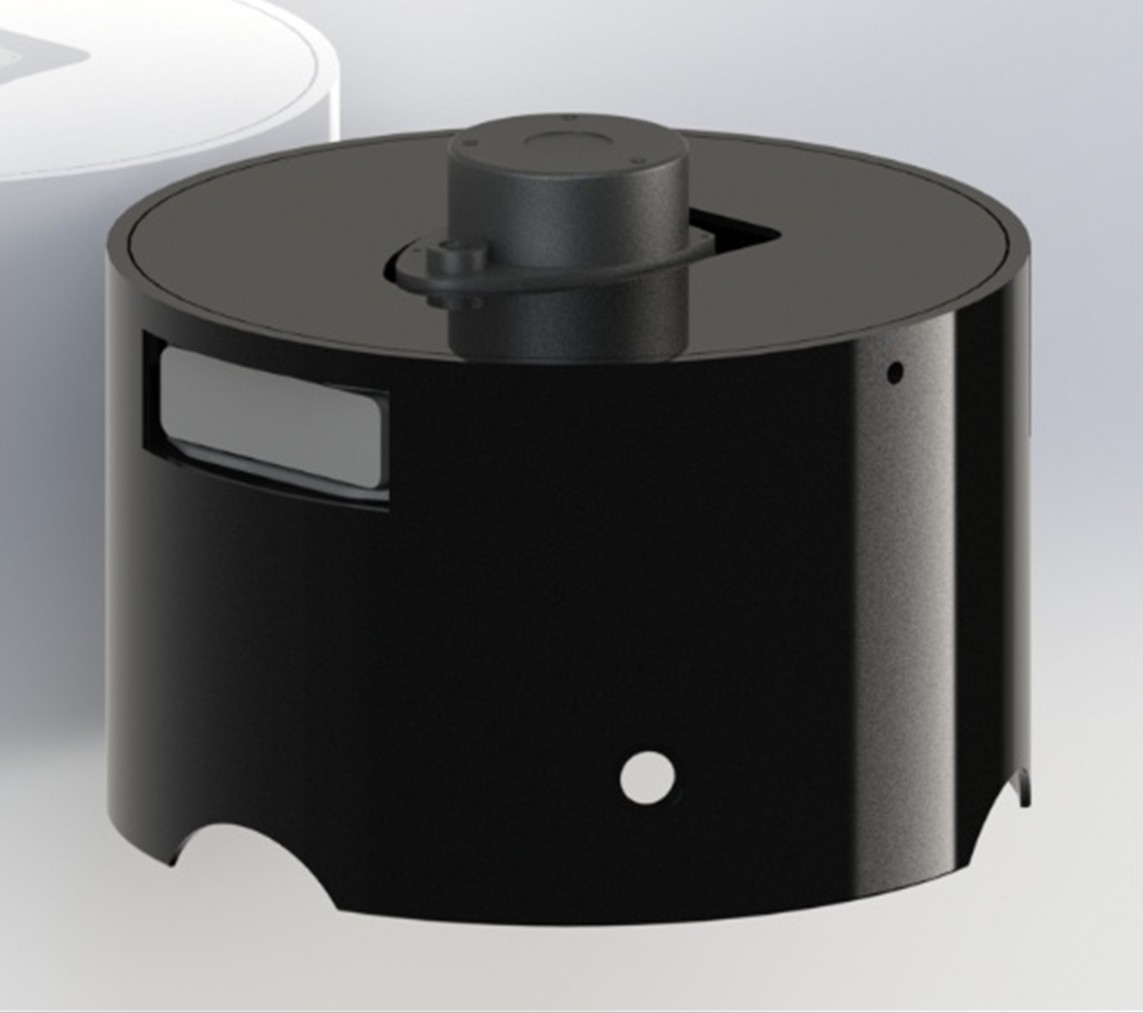
\includegraphics[width=\linewidth]{figures/Chapter 3/3d_printed_enclosure_v3.jpg}
        \caption{Assembled}
    \end{subfigure}
    \caption{Protective Enclosure Design}
    \label{fig:enclosure}
\end{figure}


\newpage
\subsection{Empirical Stress Analysis}
Currently, after selecting the material for the plates of the robot it found that there is two available thicknesses of the same material which are (3mm, 6mm).
We needed to examine all the differences between them by doing stress analysis on each one of them and compare the results. By using the engineering sense, it says that the (6mm) thickness will be better to be used but we needed to make sure if it worthy enough according to the cost and the extra weight.
\begin{itemize}
    \item \textbf{Material:} Acrylic (medium-high impact)
    \item \textbf{Dimensions:} $\phi$260
    \item \textbf{Load:} 50 N
\end{itemize}

\subsubsection{Acrylic Plate of thickness (3mm)}
\begin{figure}[H]
    \centering
    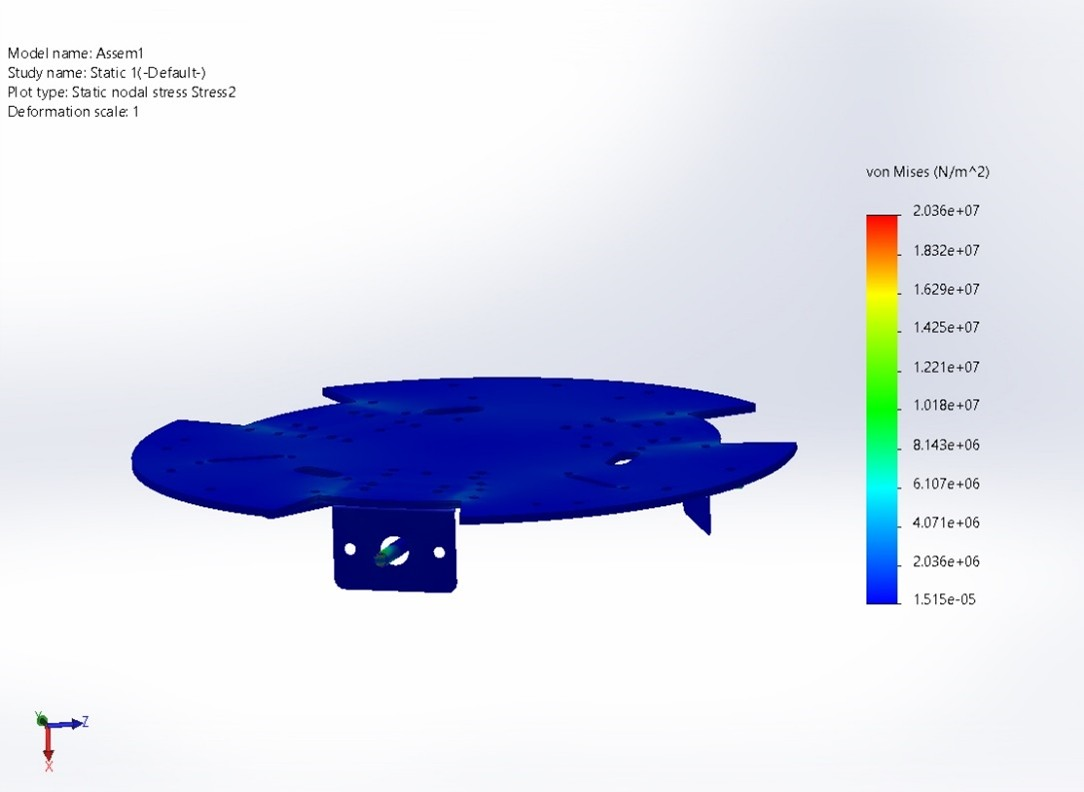
\includegraphics[width=\linewidth]{figures/Chapter 3/Von_mises_Stress3mm.jpg}
    \caption{Von Mises Stress (3mm)}
\end{figure}
\begin{figure}[H]
    \centering
    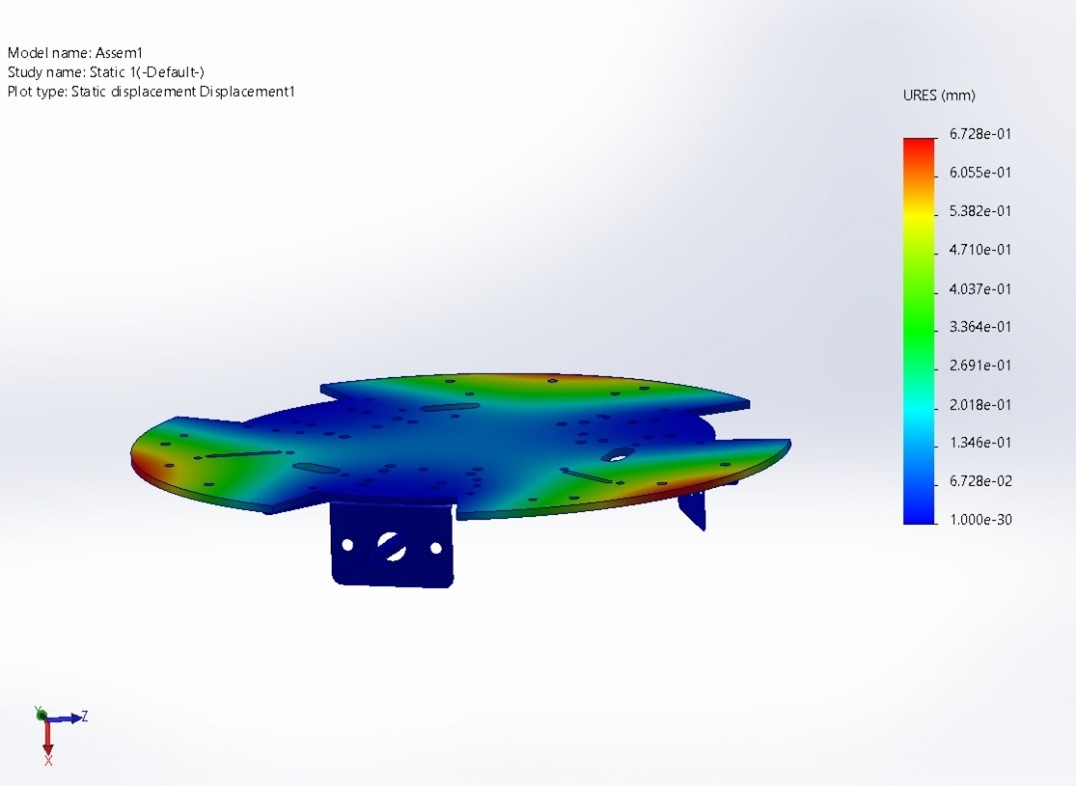
\includegraphics[width=0.85\linewidth]{figures/Chapter 3/Displacement3mm.jpg}
    \caption{Displacement (3mm)}
\end{figure}
\begin{figure}[H]
    \centering
    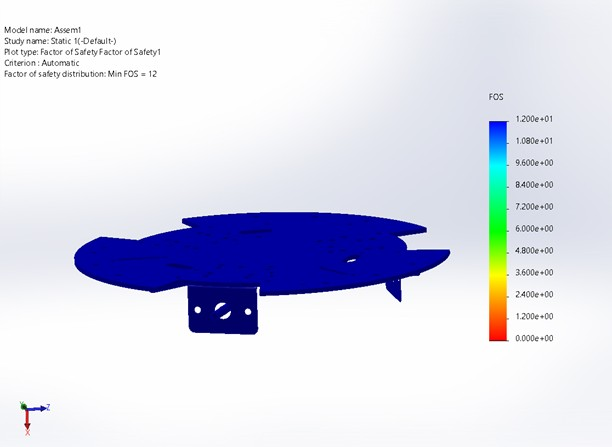
\includegraphics[width=0.85\linewidth]{figures/Chapter 3/Safety_factor3mm.jpg}
    \caption{Safety Factor (3mm)}
\end{figure}

\subsubsection{Acrylic Plate of (6mm)}
\begin{figure}[H]
    \centering
    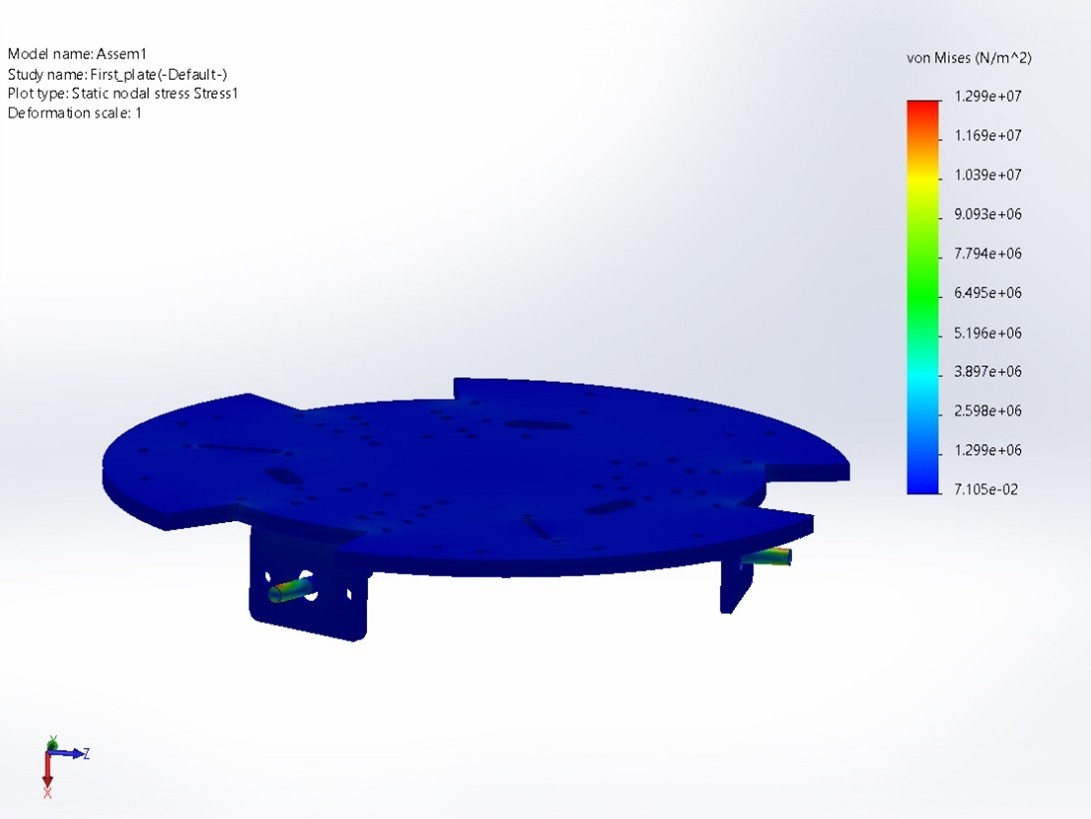
\includegraphics[width=0.75\linewidth]{figures/Chapter 3/Von_mises_Stress6mm.jpg}
    \caption{Von Mises Stress (6mm)}
\end{figure}
\begin{figure}[H]
    \centering
    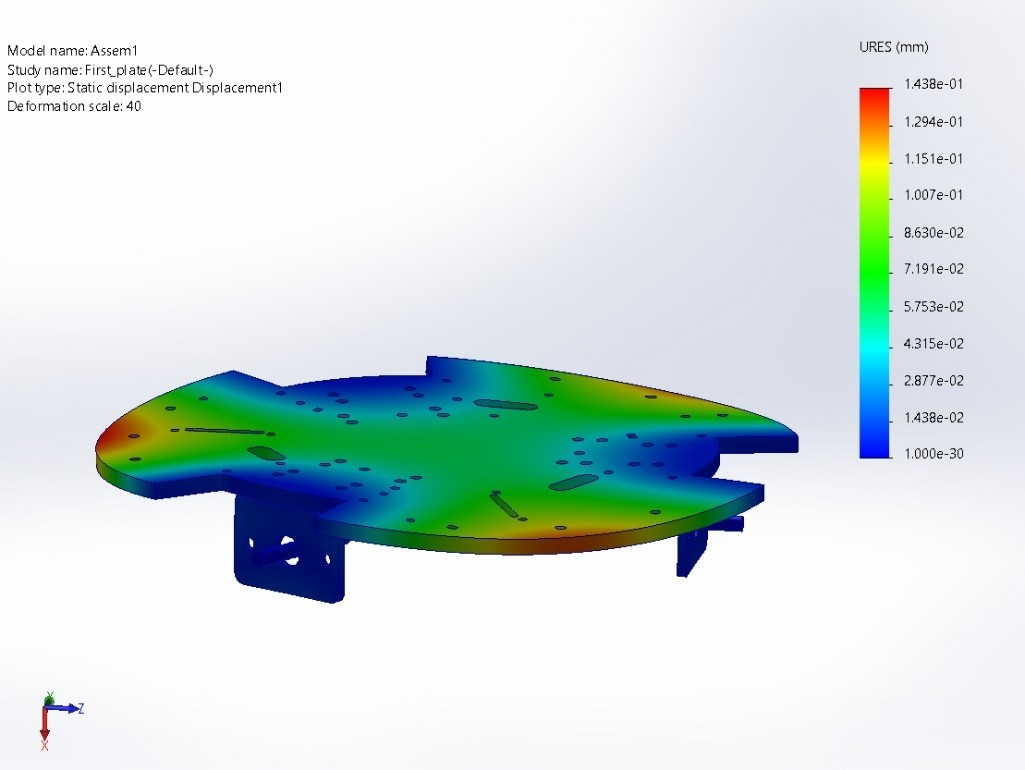
\includegraphics[width=0.75\linewidth]{figures/Chapter 3/Displacement6mm.jpg}
    \caption{Displacement (6mm)}
\end{figure}
\begin{figure}[H]
    \centering
    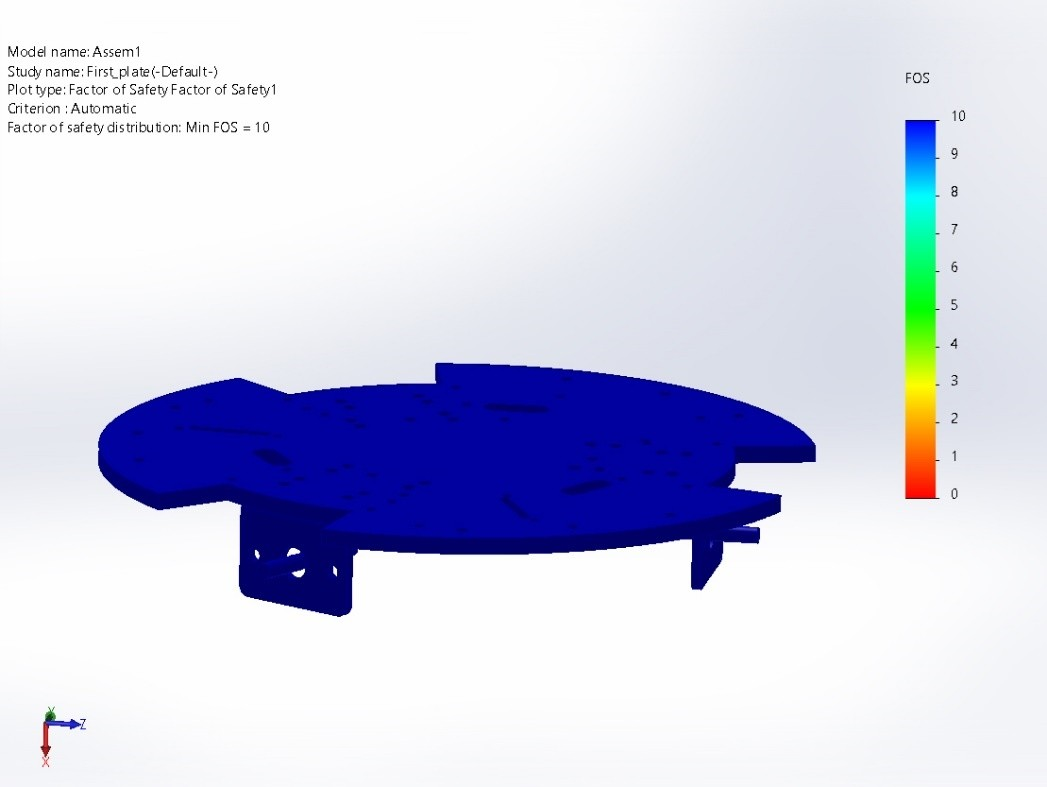
\includegraphics[width=\linewidth]{figures/Chapter 3/Safety_factor6mm.jpg}
    \caption{Safety Factor (6mm)}
\end{figure}

\subsubsection{Comparison Table}
\begin{table}[H]
\centering
\caption{Comparison of 3mm vs 6mm Acrylic}
\label{tab:acrylic_comparison}
\begin{tabular}{|l|c|c|}
\hline
\textbf{Metric} & \textbf{Acrylic Plate (3mm)} & \textbf{Acrylic Plate (6mm)} \\ \hline
Weight (gm) & 160 & 330 \\ \hline
Von Mises Stress (MPa) & 21 & 12 \\ \hline
Displacement (mm) & 0.7 & 0.145 \\ \hline
Safety Factor & 10 & 10 \\ \hline
\end{tabular}
\end{table}

Based on the Empirical Stress Analysis we conclude that the Acrylic of (6mm) thickness is the more effective thickness to be used as it’s Stronger, more durable and less in deflection in the plate to ensure the good motion of the robot without any vibrations and ensuring the wheel has more contact with the ground.


\newpage
\subsubsection{All Three layers Stress Analysis}
\begin{itemize}
    \item \textbf{Material:} Acrylic (medium-high impact)
    \item \textbf{Dimensions:} $\phi$260x6mm
    \item \textbf{Load:} 50 N
\end{itemize}
Specifying each weight of each component as a load on the point of fixation on the robot to get the more accurate results could be got.

\begin{figure}[H]
    \centering
    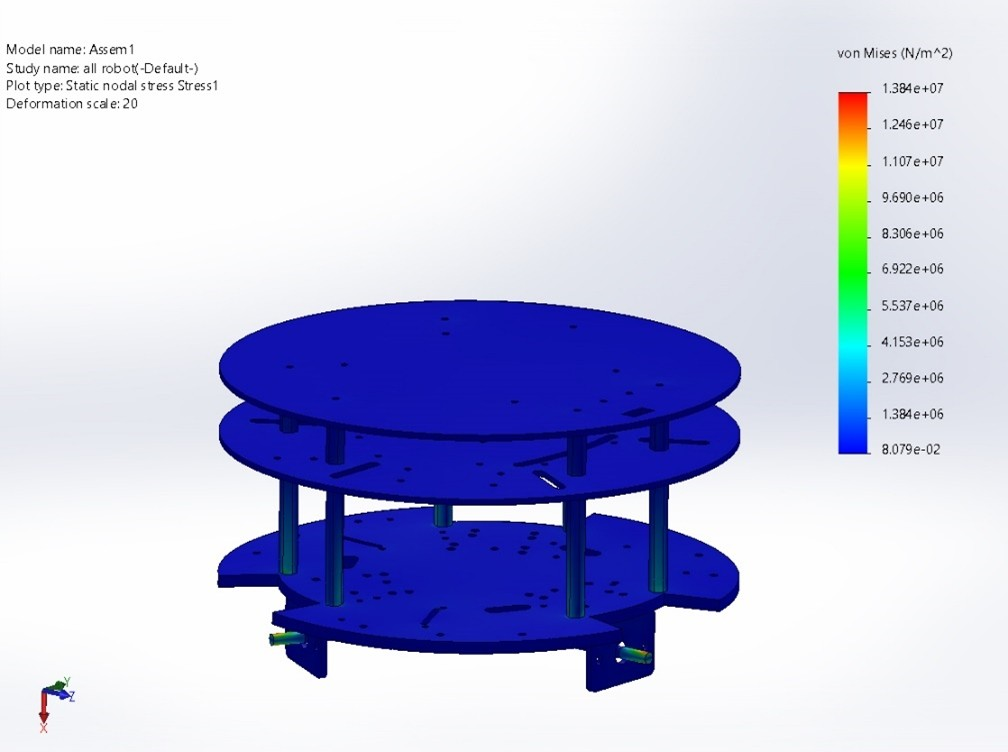
\includegraphics[width=\linewidth]{figures/Chapter 3/plate_assembly_Von_Mises_Stress.jpg}
    \caption{Full Assembly Von Mises Stress}
\end{figure}

\begin{figure}[H]
    \centering
    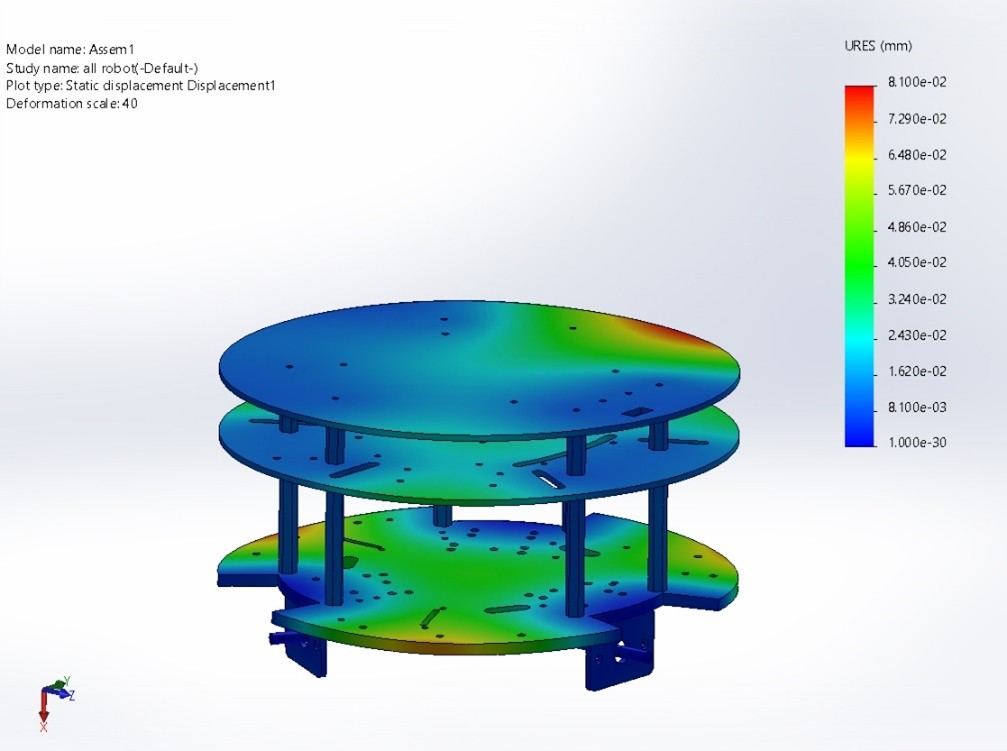
\includegraphics[width=0.7\linewidth]{figures/Chapter 3/plate_assembly_displacement.jpg}
    \caption{Full Assembly Displacement}
\end{figure}

\begin{figure}[H]
    \centering
    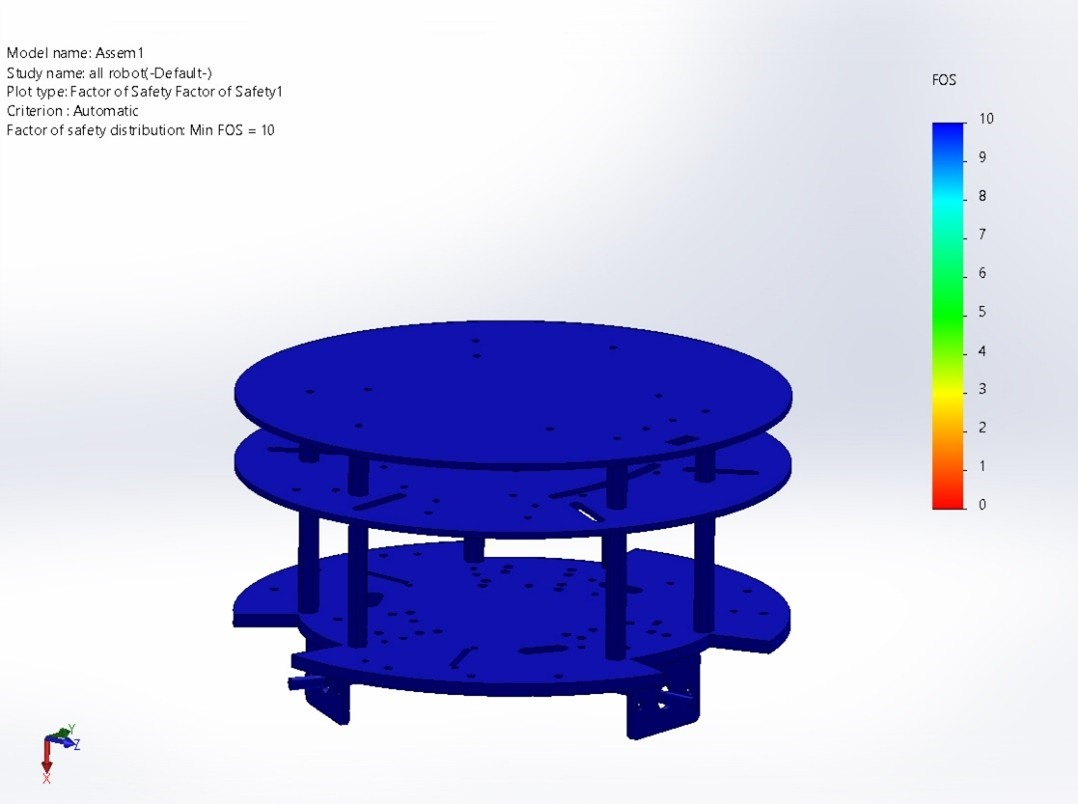
\includegraphics[width=0.7\linewidth]{figures/Chapter 3/plate_assembly_safety_factor.jpg}
    \caption{Full Assembly Safety Factor}
\end{figure}

The structural analysis confirms that the mechanical design is fully optimized for the project requirements. according to the results the chassis is durable enough to withstand more than it's designed for, ensuring minimal displacement to ensure that the kinematics of the 3-omni-wheel system remain accurate for odometry. In summary, the mechanical assembly is verified as safe, stable, and ready for manufacturing phase.

\section{Kinematic Modeling and URDF Generation}
\label{sec:urdf_generation}

The transition from a high-fidelity static SolidWorks assembly to a dynamic, simulation-ready robot is a defining phase in the development of the AUSRA swarm robots. In the context of modern mechatronics, the Unified Robot Description Format (URDF) serves as the ``single source of truth'' for the robot's physical properties, kinematic chains, and visual representation.

\subsection{Kinematic Tree Construction and Geometric Pre-processing}

The transformation of the CAD model into a functional URDF began within SolidWorks using the \texttt{sw2urdf} exporter plugin. However, for a 3-wheel omnidirectional drive, simply exporting the geometry is insufficient. To ensure the resulting model accurately reflected the physical constraints of the 120° radial symmetry, a rigorous pre-processing phase was conducted.

A robotic system is essentially a collection of ``Links'' (rigid bodies) connected by ``Joints'' (rotational or translational pivots). For the AUSRA robot, a hierarchical ``tree'' was established, starting with the \texttt{base\_link} as the root.

\begin{figure}[H]
    \centering
    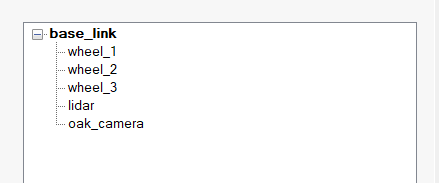
\includegraphics[width=0.85\textwidth]{figures/Chapter 5/Joints_solidworks.png}
    \caption{URDF Joint Definition in SolidWorks}
    \label{fig:joints_solidworks}
\end{figure}

To ensure precision of the kinematic transforms (TF), manual reference points were established at the geometric center of every motor shaft, wheel, and sensor. For each omni-wheel, a specific rotational axis was defined to pass through these points, serving as the pivot for the continuous joints.

A critical step was the creation of custom coordinate frames for each link, meticulously aligned such that the X, Y, and Z axes strictly adhered to the Denavit-Hartenberg (D-H) parameters. This manual alignment ensures that the ROS 2 TF tree correctly maps linear and angular velocities to the physical wheel orientations without geometric drift or mathematical singularities during runtime.

As shown in the URDF tree, the parent link specified was the \texttt{base\_link} which consists of the external body, the cover, and the base plate of the robot. The other links are all child links to the base link. Internal components not critical for simulation locomotion were omitted to keep the package lightweight for Gazebo simulation.

\begin{figure}[H]
    \centering
    \begin{subfigure}[b]{0.48\textwidth}
        \centering
        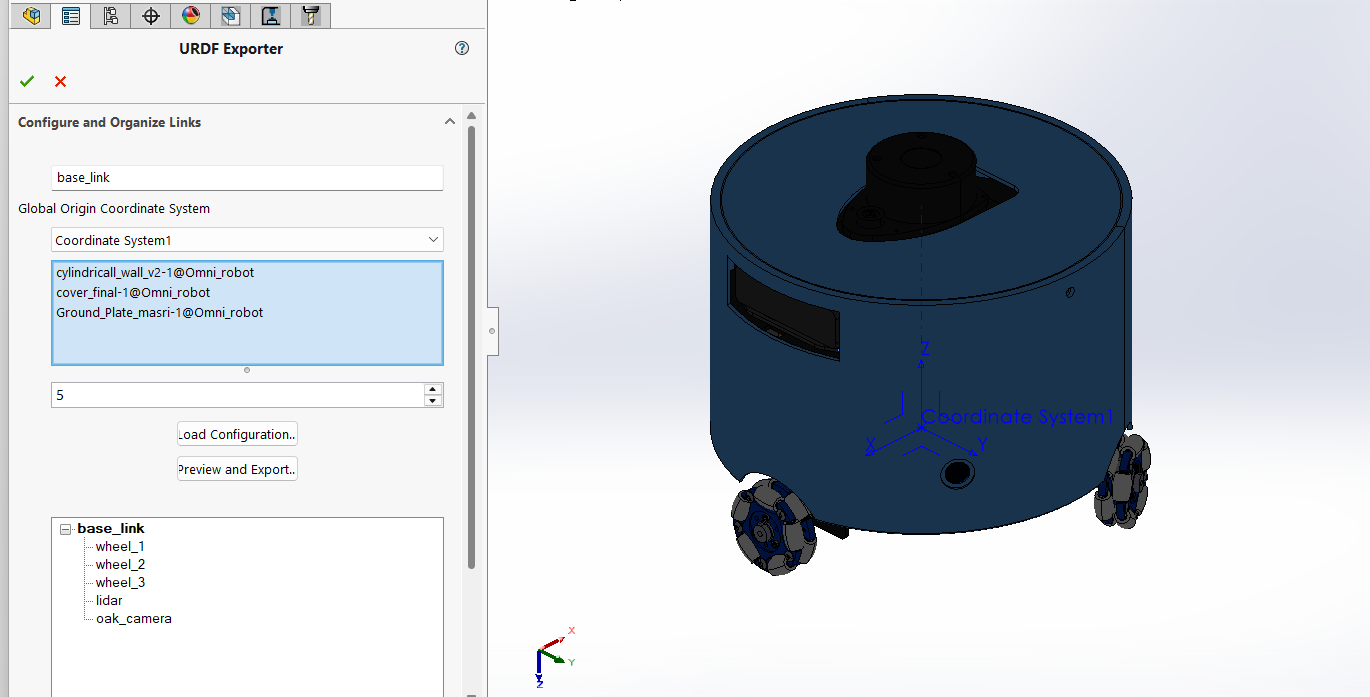
\includegraphics[width=\textwidth]{figures/Chapter 5/frames_gazebo_v1.png}
        \caption{Base Link Frame Definition}
        \label{fig:frames_gazebo_v1}
    \end{subfigure}
    \hfill
    \begin{subfigure}[b]{0.48\textwidth}
        \centering
        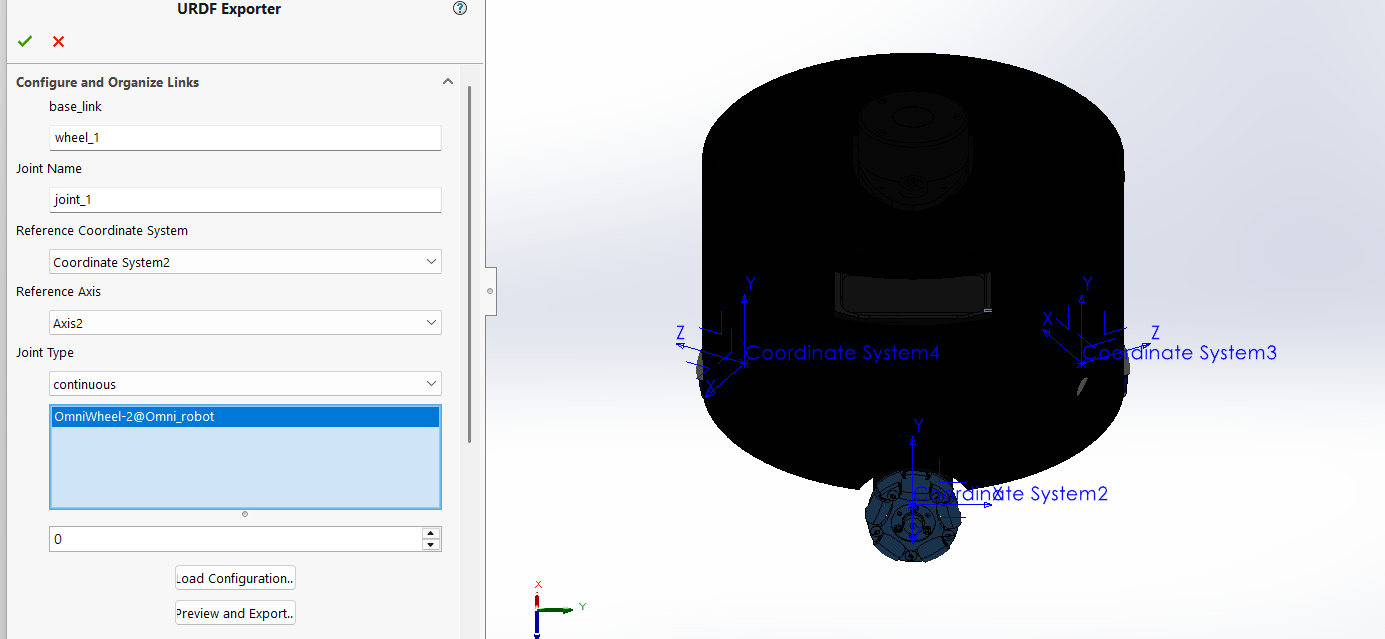
\includegraphics[width=\textwidth]{figures/Chapter 5/Frames_gazebo_v2.png}
        \caption{Wheel Frame Alignment}
        \label{fig:frames_gazebo_v2}
    \end{subfigure}
    \caption{Coordinate Frame Definition in Gazebo}
    \label{fig:frames_gazebo}
\end{figure}

For an omnidirectional platform, this alignment is vital; the Z-axis of each wheel must be perfectly perpendicular to the Z-axis of the \texttt{base\_link} coordinate frame and perpendicular to the wheel side face, while the X-axis must align with the forward translation vector of that specific wheel. Each wheel has its coordinate frame and axis specified with joint type set to \texttt{continuous}.

\begin{figure}[H]
    \centering
    \begin{subfigure}[b]{0.48\textwidth}
        \centering
        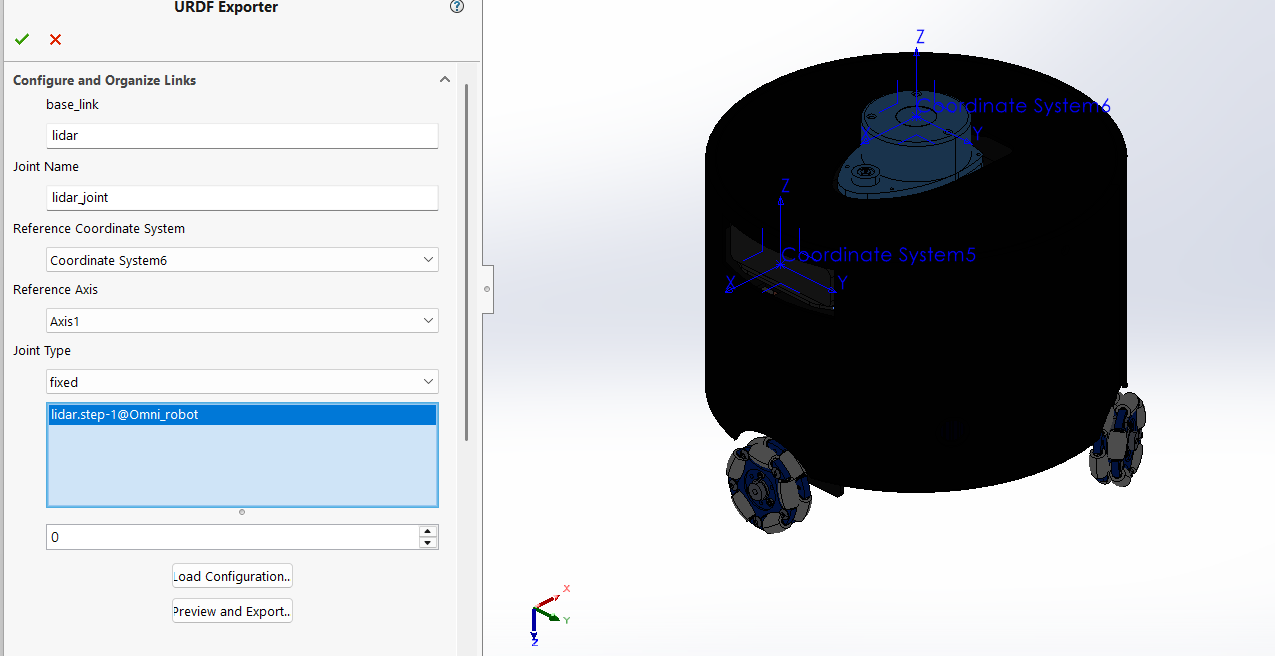
\includegraphics[width=\textwidth]{figures/Chapter 5/Frames_gazebo_v3.png}
        \caption{LiDAR and Camera Link Placement}
        \label{fig:frames_gazebo_v3}
    \end{subfigure}
    \hfill
    \begin{subfigure}[b]{0.48\textwidth}
        \centering
        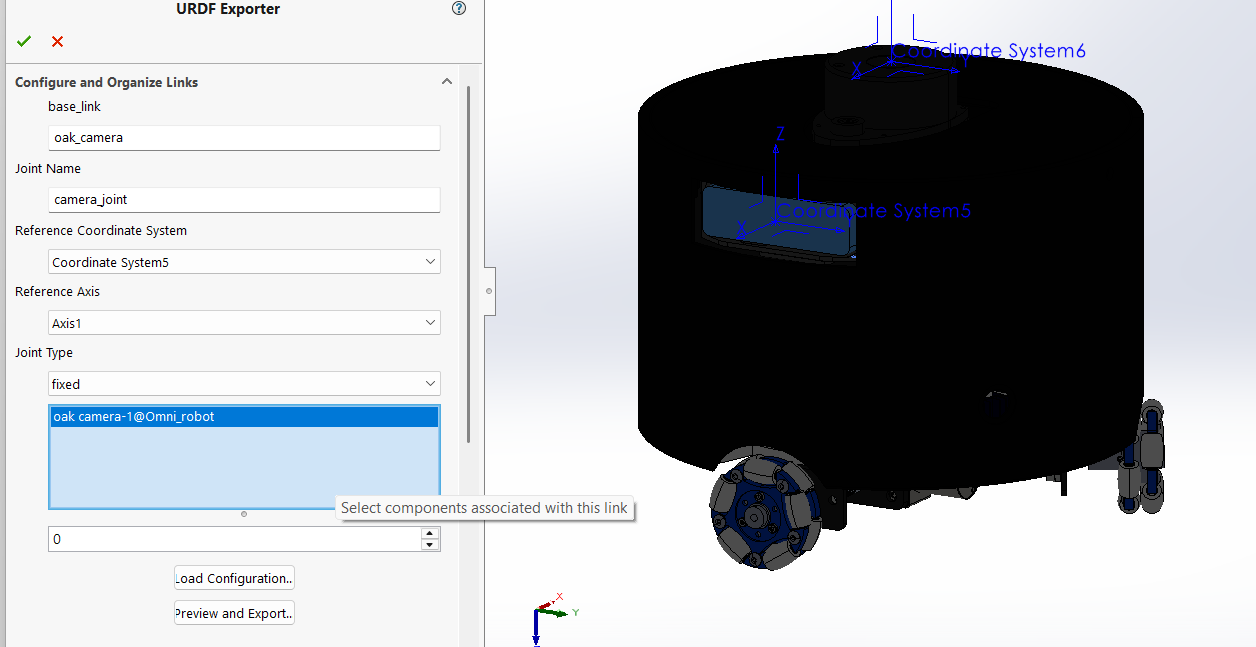
\includegraphics[width=\textwidth]{figures/Chapter 5/Frames_gazebo_v4.png}
        \caption{Complete TF Tree Visualization}
        \label{fig:frames_gazebo_v4}
    \end{subfigure}
    \caption{Sensor Link Definition}
    \label{fig:sensor_frames}
\end{figure}

The LiDAR link and OAK-D camera link are specified in the URDF for accurate placement when plugins are added for Gazebo simulation testing and code verification. The joint types of these sensor links are \texttt{fixed}.

\subsection{ROS 2 Migration and Package Reconfiguration}

Once the reference geometry and kinematic relationships were finalized, the robot was exported as a unified package. However, a significant technical hurdle was encountered: the standard exporter plugin is natively designed for the legacy ROS 1 environment. This resulted in a directory structure, metadata, and launch logic that were entirely incompatible with the ROS 2 Humble stack and its \texttt{ament\_cmake} build system.

To resolve this, a comprehensive reconfiguration of the exported package was undertaken:

\subsubsection{Build System Adaptation}

The \texttt{package.xml} was rewritten to include modern ROS 2 dependencies such as \texttt{robot\_state\_publisher}, \texttt{joint\_state\_publisher}, and \texttt{xacro}. Simultaneously, the \texttt{CMakeLists.txt} was reconstructed to utilize the \texttt{ament\_package()} macros, ensuring the meshes and URDF files were correctly indexed during the \texttt{colcon build} process.

\subsubsection{Launch System Development}

In ROS 2, launch files are Python-based scripts that manage the lifecycle and parameters of multiple nodes. New launch files were developed for two primary tasks:

\paragraph{RViz2 Visualization}
A launch script was created to load the URDF, start the \texttt{robot\_state\_publisher}, and open RViz2 with a pre-configured view. This allows real-time verification of the transform frames (TF), ensuring the OAK-D camera and LiDAR are spatially aligned with the robot's center.

\begin{figure}[H]
    \centering
    \begin{subfigure}[b]{0.48\textwidth}
        \centering
        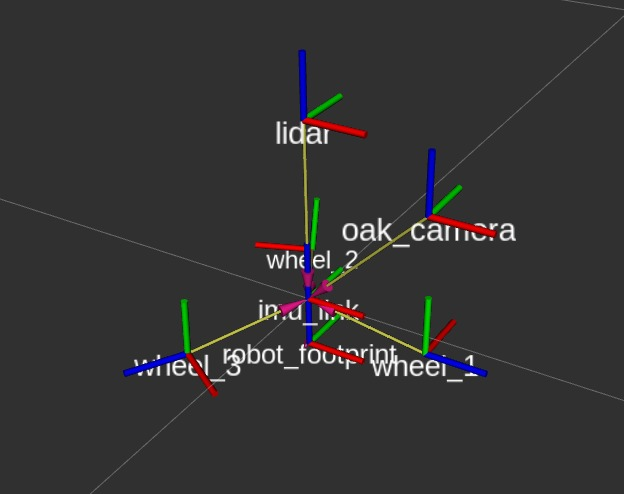
\includegraphics[width=\textwidth]{figures/Chapter 5/Frames_axis_rviz2.jpeg}
        \caption{TF Frames in RViz2}
        \label{fig:frames_rviz1}
    \end{subfigure}
    \hfill
    \begin{subfigure}[b]{0.48\textwidth}
        \centering
        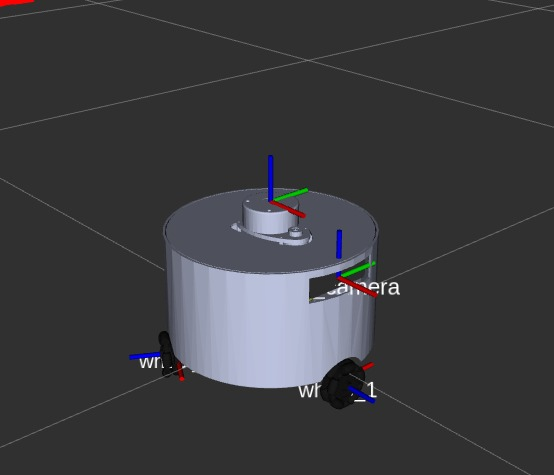
\includegraphics[width=\textwidth]{figures/Chapter 5/Frames_axis_rviz_1.jpeg}
        \caption{Robot Model Visualization}
        \label{fig:frames_rviz2}
    \end{subfigure}
    \caption{URDF Visualization in RViz2}
    \label{fig:rviz_visualization}
\end{figure}

\paragraph{Gazebo Simulation}
A secondary launch file was engineered to ``spawn'' the robot within the Gazebo physics engine. This required converting the URDF into an SDF (Simulation Description Format) on the fly and integrating Gazebo-specific plugins for the camera, IMU, LiDAR, and the omnidirectional wheel controller.

\begin{figure}[H]
    \centering
    \begin{subfigure}[b]{0.48\textwidth}
        \centering
        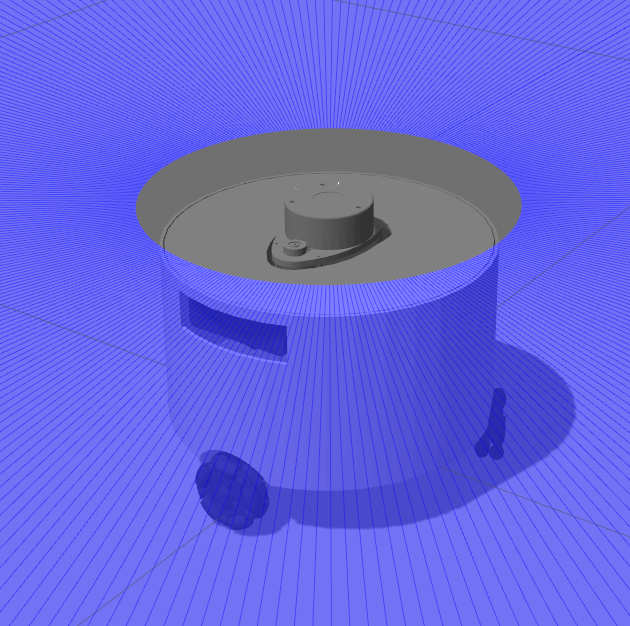
\includegraphics[width=\textwidth]{figures/Chapter 5/Robot_gazebo1.png}
        \caption{Robot Spawned in Gazebo}
        \label{fig:robot_gazebo1}
    \end{subfigure}
    \hfill
    \begin{subfigure}[b]{0.48\textwidth}
        \centering
        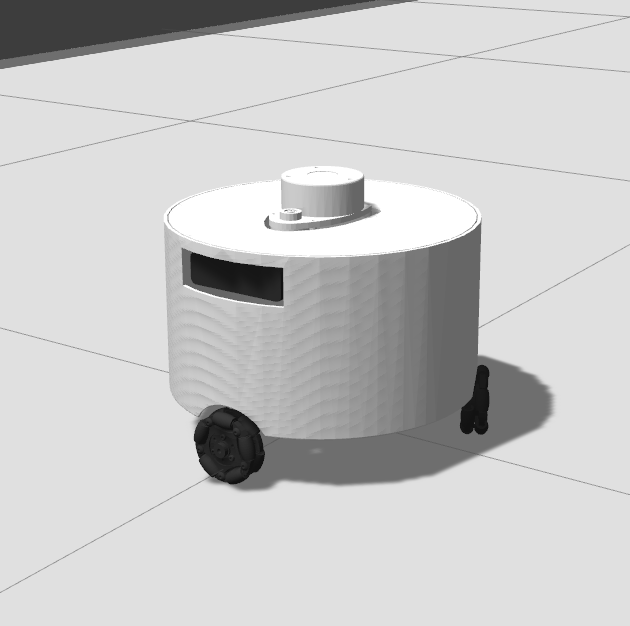
\includegraphics[width=\textwidth]{figures/Chapter 5/Robot_gazebo2.png}
        \caption{Physics Simulation Active}
        \label{fig:robot_gazebo2}
    \end{subfigure}
    \caption{AUSRA Robot in Gazebo Simulation}
    \label{fig:gazebo_simulation}
\end{figure}

\subsubsection{Inertial and Visual Optimization}

To ensure realistic behavior in simulation, the \texttt{<inertial>} tags for each link were populated using the exact mass and ``Inertia Tensor'' values calculated by SolidWorks' Mass Properties tool. Furthermore, the visual meshes were optimized and exported as \texttt{.stl} files, providing high-fidelity visual representation in RViz2 while maintaining low computational overhead.

\subsection{Summary}

The final result of this process is a robust and dynamic-ready model of the AUSRA robot that can be spawned in the Gazebo environment. This is the foundational step for any autonomous robot project. The reconfigured package serves as the bridge between the mechanical design and the high-level autonomous navigation algorithms, allowing the research team to test swarm coordination and SLAM algorithms in a high-fidelity simulation environment before deploying the physical robots---significantly reducing the risk of hardware damage during the development of complex 2D mapping behaviors.
